\documentclass[a4paper,10pt]{article}
\usepackage[utf8]{inputenc}
\usepackage[a4paper,
            bindingoffset=0.2in,
            left=1in,
            right=1in,
            top=1in,
            bottom=1in,
            footskip=.25in]{geometry}

%###############################################################################

%\input{~/layout/global_layout}


%###############################################################################

% packages begin

\usepackage[
  backend=biber,
  sortcites=true,
  style=alphabetic,
  eprint=true,
  backref=true
]{biblatex}
\addbibresource{bibliographie.bib}
\usepackage[acronym]{glossaries}

\usepackage{euscript}[mathcal]
% e.g. \mathcal{A} for fancy letters in mathmode
\usepackage{amsmath,amssymb,amstext,amsthm}

\usepackage{mdframed}
\newmdtheoremenv[nobreak=true]{problem}{Problem}[subsection]
\newmdtheoremenv[nobreak=true]{claim}{Claim}[subsection]
\newtheorem{definition}{Definition}[subsection]
\newtheorem{lemma}{Lemma}[claim]
\newtheorem{plemma}{Lemma}[problem]

\usepackage{mathtools}
\DeclarePairedDelimiter\ceil{\lceil}{\rceil}
\DeclarePairedDelimiter\floor{\lfloor}{\rfloor}

\usepackage{enumerate}
\usepackage[pdftex]{graphicx}
\usepackage{subcaption}
% 'draft' für schnelleres rendern mitübergeben -> [pdftex, draft]
% dadruch wird nicht das bild mitgerendered, sondern nur ein kasten mit bildname -> schont ressourcen

\usepackage{hyperref}

\usepackage{tikz}
\usetikzlibrary{arrows,automata,matrix,positioning,shapes}

% for adding non-formatted text to include source-code
\usepackage{listings}
\lstset{language=Python,basicstyle=\footnotesize}
% z.B.:
% \lstinputlisting{source_filename.py}
% \lstinputlisting[lanugage=Python, firstline=37, lastline=45]{source_filename.py}
%
% oder
%
% \begin{lstlisting}[frame=single]
% CODE HERE
%\end{lstlisting}
\usepackage{algorithm}
\usepackage{algpseudocode}

\usepackage{wasysym}

\usepackage{titling}
\usepackage{titlesec}
\usepackage[nocheck]{fancyhdr}
\usepackage{lastpage}

\usepackage{kantlipsum}
\usepackage[colorinlistoftodos,prependcaption,textsize=tiny]{todonotes}

% packages end
%###############################################################################

\pretitle{% add some rules
  \begin{center}
    \LARGE\bfseries
} %, make the fonts bigger, make the title (only) bold
\posttitle{%
  \end{center}%
  %\vskip .75em plus .25em minus .25em% increase the vertical spacing a bit, make this particular glue stretchier
}
\predate{%
  \begin{center}
    \normalsize
}
\postdate{%
  \end{center}%
}

\titleformat*{\section}{\Large\bfseries}
\titleformat*{\subsection}{\large\bfseries}
\titleformat*{\subsubsection}{\normalsize\bfseries}

\titleformat*{\paragraph}{\Large\bfseries}
\titleformat*{\subparagraph}{\large\bfseries}

%###############################################################################
% TODO define Headers and Fotter

\pagestyle{fancy}
\fancyhf{}
% l=left, c=center, r=right; e=even_pagenumber, o=odd_pagenumber; h=header, f=footer
% example: [lh] -> left header, [lof,ref] -> fotter left when odd, right when even
%\fancyhf[lh]{}
%\fancyhf[ch]{}
%\fancyhf[rh]{}
%\fancyhf[lf]{}
\fancyhf[cf]{\footnotesize Page \thepage\ of \pageref*{LastPage}}
%\fancyhf[rf]{}
\renewcommand{\headrule}{} % removes horizontal header line

% Fotter options for first page

\fancypagestyle{firstpagestyle}{
  \renewcommand{\thedate}{\textmd{}} % removes horizontal header line
  \fancyhf{}
  \fancyhf[lh]{\ttfamily M.Sc. Computer Science\\KTH Royal Institute of Technology}
  \fancyhf[rh]{\ttfamily Period 3\\\today}
  \fancyfoot[C]{\footnotesize Page \thepage\ of \pageref*{LastPage}}
  \renewcommand{\headrule}{} % removes horizontal header line
}
%###############################################################################

\newcommand\extrafootertext[1]{%
    \bgroup
    \renewcommand\thefootnote{\fnsymbol{footnote}}%
    \renewcommand\thempfootnote{\fnsymbol{mpfootnote}}%
    \footnotetext[0]{#1}%
    \egroup
}

%###############################################################################

\title{
  \normalsize{DD2358 VT25 Introduction to}\\
  \normalsize{High Performance Computing}\\
  \large{Project Report: Optimizing Finite-Volume Fluid Simulation}
}
\author{
  \small Rishi Vijayvargiya\textsuperscript{\textdagger}\\[-0.75ex]
%  \footnotesize\texttt{MN: }\\[-1ex]
  \scriptsize\texttt{rishiv@kth.se}
  \and
  \small Paul Mayer\textsuperscript{\textdagger}\\[-0.75ex]
%  \footnotesize\texttt{MN: }\\[-1ex]
  \scriptsize\texttt{pmayer@kth.se}
}
\date{}

%###############################################################################
% define Commands

\newcommand{\N}{\mathbb{N}}
\newcommand{\R}{\mathbb{R}}
\newcommand{\Z}{\mathbb{Z}}
\newcommand{\I}{\mathbb{I}}

\newcommand{\E}{\mathbb{E}}
\newcommand{\Prob}{\mathbb{P}}

\renewcommand{\epsilon}{\varepsilon}

% Todo: Set Counter to Excercise Sheet Number
%\setcounter{section}{1}
%\setcounter{subsection}{1}

%###############################################################################
\makeatletter
\renewcommand*{\@fnsymbol}[1]{\ensuremath{\ifcase#1\or \dagger\or \ddagger\or
   \mathsection\or \mathparagraph\or \|\or **\or \dagger\dagger
   \or \ddagger\ddagger \else\@ctrerr\fi}}
\makeatother
%###############################################################################

\begin{document}
\maketitle
\extrafootertext{\textsuperscript{\textdagger}Authors made equal contribution to the project}
\thispagestyle{firstpagestyle}

% \tableofcontents
\listoftodos
\vspace{1em}

% content begin
%

\section*{Prefix}
The code for our project can be found at this location: \url{https://github.com/paulmyr/DD2358-HPC25/tree/master/10_project_rishi_paul}. The original code for this project is taken from the following \href{https://github.com/pmocz/finitevolume-python/blob/master/finitevolume.py}{GitHub repository}.
The code is written by \href{https://pmocz.github.io}{Philip Mocz}.\\

We expect to get a grade of \textbf{A} (for the project and the course).
Finally, we made following changes before starting with the project:
\begin{itemize}
  \item Fixed a bug that resulted in an infinite loop when setting the \verb|plotRealTime| flag to \verb|False|.
\end{itemize}

\tableofcontents
\newpage
\section{Introduction}
The Kelvin-Helmholz-Inequality is a phenomenom that arises when two fluid layers of different velocities interface with each other.
It results in characteristic patterns that can be observered, e.g. in clouds, the surface of the sun or in jupyters colorful atmosphere.
Philip Mocz created an which produces a visualization of the characteristic swirls of the K-H-inequality.

The Finite Volume method is a popular simulation technique to simulate fluids or partial differential equations that can be represented in a conservative form.
This is often the case for equations that describe physical conservation laws.
The Euler-Fluid-Equations (a simplifications of the Navier-Stokes-Equations) can be represented --- besides it's primitive description --- in such conservative form.
Within the algorithm, Philip Mosz makes use of both representations of the formula.
He uses the primitive form to extrapolate values in time and space, but uses the conservative representation to derive the update formula.
Numerically, this achieves the best of both worlds.
Extrapolating within the primitive form is more stable whereas the conservative representation is used to compute the update efficiently.

The algorithm in principle works as follows:
For each timestep and each cell do
\begin{enumerate}
  \item Get cell central primitive variables (convert from conservative ones)
  \item Calculate timestep size $\Delta t$
  \item Calculate gradient using primitive variables (using central differences)
  \item Extrapolate primitive variables in time
  \item Extrapolate primitive variables to faces
  \item Compute fluxes along each face
  \item Update solution by adding fluxes to conservative variables
\end{enumerate}

First it is important to note, that all of these steps are computed for the density $\rho$, pressure $p$ as well as the velocity in both dimensions $v_x$ and $v_y$.
These computations don't rely on each other and can therefore be performed in parallel.

Second, each function call in itself usually performs a computation on the whole grid.
The original implementation makes use of this by vectorizing the computation (e.g. using \verb|np.roll|).
These calculations can be parallelized --- they are in fact embarassingly parallel.

We aim to introduce optimizations that decrease the overall runtime of the computation.
To achieve this, we use techniques obtained from the lectures, specifically using cython to use precompiled c code to reduce python overhead and investigate a distributed computation approach utilizing dask.
As a little bonus treat, we combined the dask and cython approach.
Lastly, we investigated using GPU accellerators using pytorch.

\section{Baseline tests}
\subsection{Testing and profiling setup}
All runtime tests that show results for a specific grid size were computed on a 2021 M1 Macbook Pro (16') if not explicity stated otherwise.
For every grid we simulated 256 time steps without computing the visualization.
Every test was run three times, runtimes were then averaged.

Some of the profiling graphs are computed on a 2020 M1 Macbook Air, we specify it explicitly when this was done so.
\todo[inline]{Do we need to include the box-plot anywhere?}
All implementations were tested to ensure correctness by comparing the final \verb|rho| values on the grid between baseline and optimized implementations.
Every approach presented in this report passed this test.

\subsection{Runtime}
We approached this problem by trying to get a basic understanding of what might be the runtime bottleneck.
For this we used the line profiler.
We simulated\footnote{using the MacBook Air (2020)} on a 256x256 grid for 256 iterations.
We came to the conclusion that a large portion (nearly 50\%) of computation time is spent to compute the fluxes (\verb|getFlux| method).
\begin{lstlisting}[language=bash,basicstyle=\scriptsize\ttfamily]
Line #      Hits         Time  Per Hit   % Time  Line Contents
==============================================================
   195                                           @profile
   196                                           def main():
[...]
   272                                               # compute fluxes (local Lax-Friedrichs/Rusanov)
   273       256     357351.0   1395.9     25.0      flux_Mass_X, flux_Momx_X, flux_Momy_X,
                                                         flux_Energy_X = getFlux(...)
   274       256     320673.0   1252.6     22.4      flux_Mass_Y, flux_Momy_Y, flux_Momx_Y,
                                                         flux_Energy_Y = getFlux(...)
[...]
\end{lstlisting}
All other function calls accumulated to the other 50\%, however each in itself were more or less neglegtable (at most below 4\%).
This strongly incentivised to focus our efforts onto this part of the computation.

The runtime of the simulation mostly depends on two parameters.
First and foremost the number of time steps:
Each time step is computed in one iteration of the main loop.
Figure \ref{fig:runtime_per_iteration} displays the runtime the computation of each timestep needs.
We can observe that the runtime per iteration is mostly consistant over the course of the simulation.
\begin{figure}[h]
  \centering
  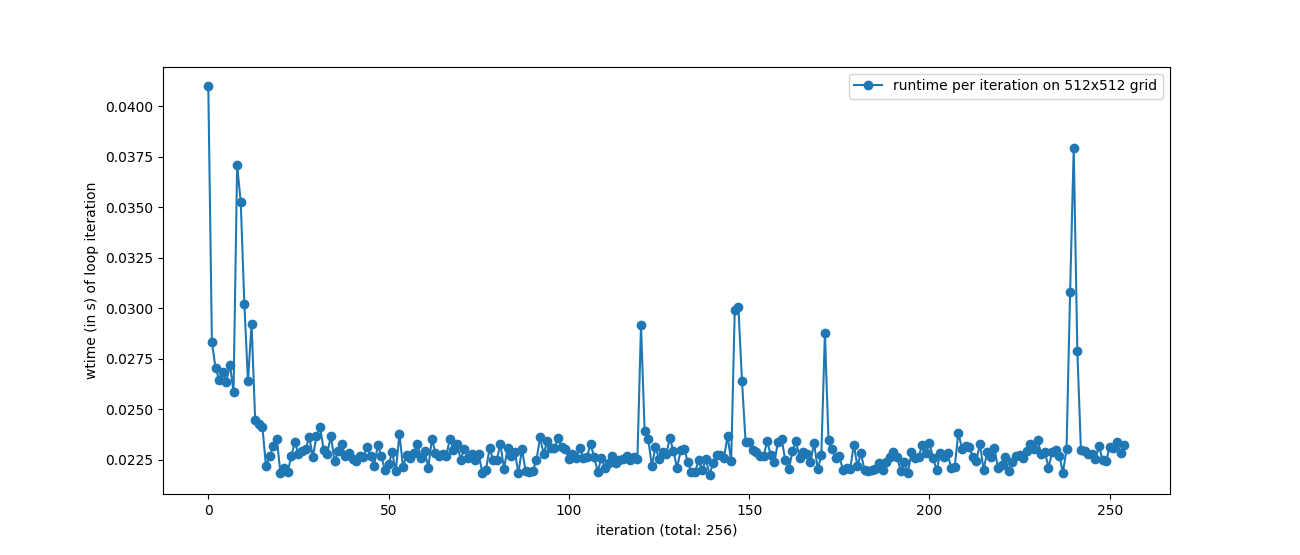
\includegraphics[width=0.7\textwidth]{images/baseline/baseline_per_iteration_macair.png}
  \caption{Baseline Runtime per iteration on 2021 macbook pro}
  \label{fig:runtime_per_iteration}
\end{figure}
Important note:
To simulate a fixed time, the total number of timesteps increases by increasing grid resolution.
With other words, simulating two seconds using a fine grid uses more iterations than simulating two seconds using a corse grid. 
The reason is that $dt$, which is computed each loop, is dependent on $dx$ --- the granularity of the mesh.

The second important parameter is the grid size.
Finer grids allow for higher precision but increase the computational complexity quadratically.
To measure runtime over a variety of gridsizes, we decided to keep the number of time steps constant.
We simulated 256 timesteps over all grid sizes and performed each computation three times, which we then averaged.
The \textit{baseline/default}\footnote{Code for baseline found \href{https://github.com/paulmyr/DD2358-HPC25/blob/master/10_project_rishi_paul/code/finitevolume_runtimeplots.py}{here}.} is the original implementation of the simulation.
\begin{figure}[h]
  \centering
  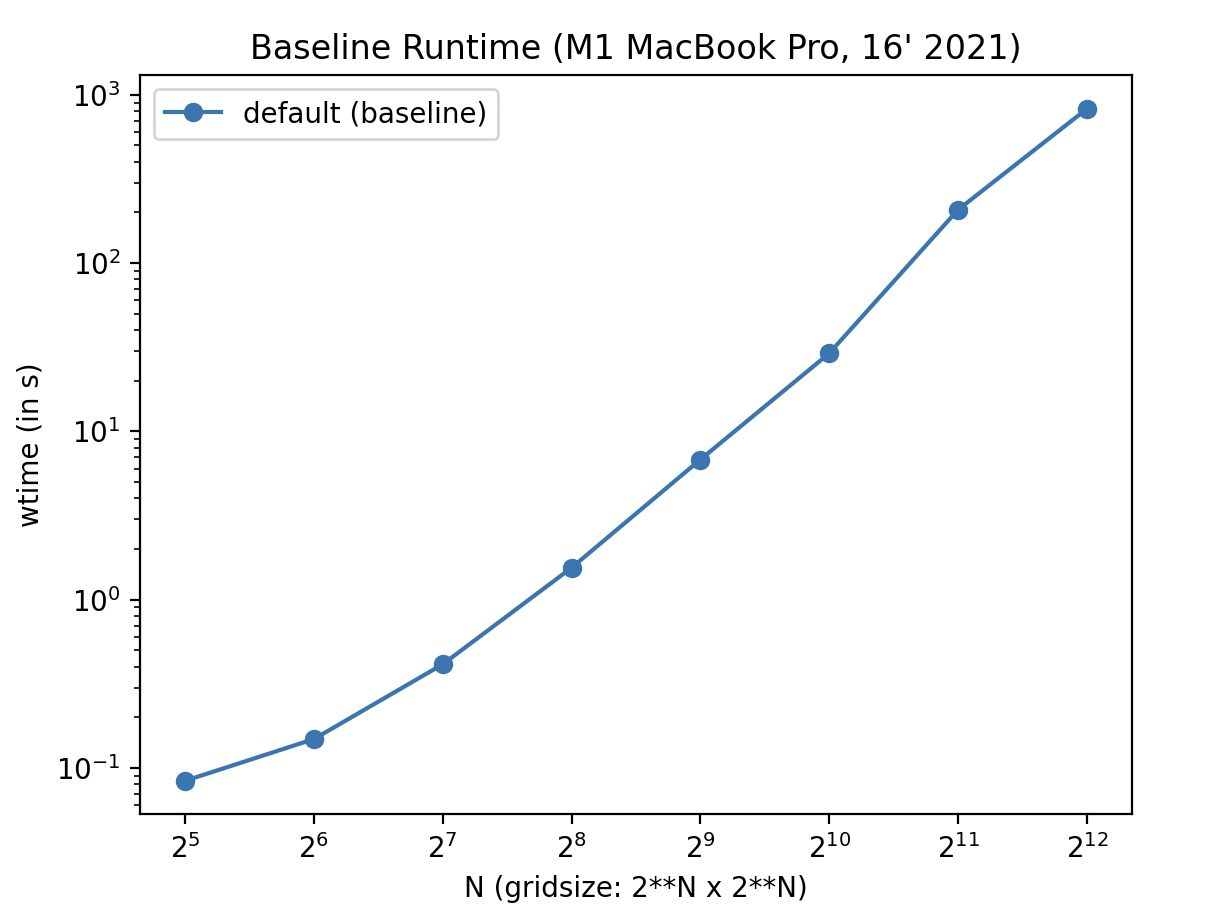
\includegraphics[width=0.7\textwidth]{images/baseline/baseline_performance.png}
  \caption{Baseline Runtime per iteration on 2021 macbook pro}
  \label{fig:runtime_baseline}
\end{figure}
Figure \ref{fig:runtime_baseline} vizualizes the walltimes for different grid sizes of the baseline implementation on a log-log scale.

\subsection{Memory}
We measured the memory consumption of the simulation over the runtime on a 512x512 grid.
Figure \ref{fig:memory_over_simulation} depicts the measurement we obtained using the mprof module in python.
We see that once all memory has been allocated, all computations are performed inplace.
This is good, since the reallocating memory and waiting for the garbage collector to free memory could lead to performance issues, especially on larger grids.

\begin{figure}[h]
  \centering
  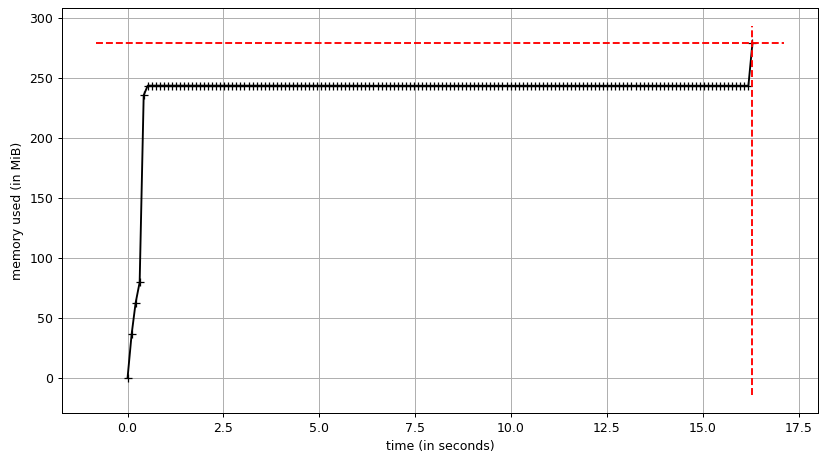
\includegraphics[width=0.7\textwidth]{images/baseline/baseline_memory_512.png}
  \caption{Memory consumption 512x512 grid measured on M1 MacBook Air}
  \label{fig:memory_over_simulation}
\end{figure}

\section{Optimizations using Cython}
Since \verb|getFlux| was the bottleneck for the simulation based on our profiling, we focused on optimizing this function using Cython.
We investigated four approaches in total, only one performed better than the baseline. \footnote{The code for this section is present in the \textit{cython/} directory of the repository \href{https://github.com/paulmyr/DD2358-HPC25/blob/master/10_project_rishi_paul/code/cython/finitevolume_cython_lib.pyx}{here}}.
All runtimes presented in this section timed the simulation using different versions of the \verb|getFlux| method.

\subsection{Attempt 1: Using \textit{np.asarray} With Minimal Changes}
For the first attempt, we extensively use Cython's \emph{typed memoryviews}; both for arguments and intermediate variables defined in the function.
The memoryviews are converted to numpy arrays using \verb|np.asarray| to allow for vectorized operations.
This way there is minimal deviation from the structure of the original code\footnote{Code found \href{https://github.com/paulmyr/DD2358-HPC25/blob/master/10_project_rishi_paul/code/cython/finitevolume_cython_lib.pyx\#L8}{here} (\textit{getFluxAsArray}).}.
Figure \ref{fig:cython_attempts} depicts the performance of this attempt compared to the baseline, which is slightly worse.
We believe this can be explained by the frequent calls to \verb|np.asarray|, which likely requires interactions with the Python runtime.
The original code was vectorized incredibly well, so there were no easy performance gains (e.g. by optimizing nested \verb|for-| loops) that Cython could have automatically achieved without our intervention.

\subsection{Attempt 2: Re-Implement Vectorized Arithmetic}
We re-implemented\footnote{Code found \href{https://github.com/paulmyr/DD2358-HPC25/blob/master/10_project_rishi_paul/code/cython/finitevolume_cython_lib.pyx\#L155}{here} (\textit{getFluxAsLoops}).} numpy's vectorized operations using simple nested \verb|for-|loops.
For example, the addition of 2 numpy arrays \verb|a + b| was re-implemented with nested \verb|for-|loops using element-wise additions.
We continued using typed memoryviews in all places.
We hoped that Cython would be able to optimize the simpler nested loops, leading to a better runtime; however, this was not the case.
The comparison of this attempt with the baseline and Attempt-1 can be seen in Figure \ref{fig:cython_attempts}. 

One explanation for the poor performance of this implementation could be attributed to the fact that each operation requires the program to iterate over the arrays multiple times.
The original code contains various combination of such simpler operations to compute the intermediate variables.
Another issue could be the fact that numpy is very good at vectorizing these optimizations, whereas the used c-compiler of cython\todo{what compiler does cython use?} might not.
\begin{figure}[h]
  \centering
  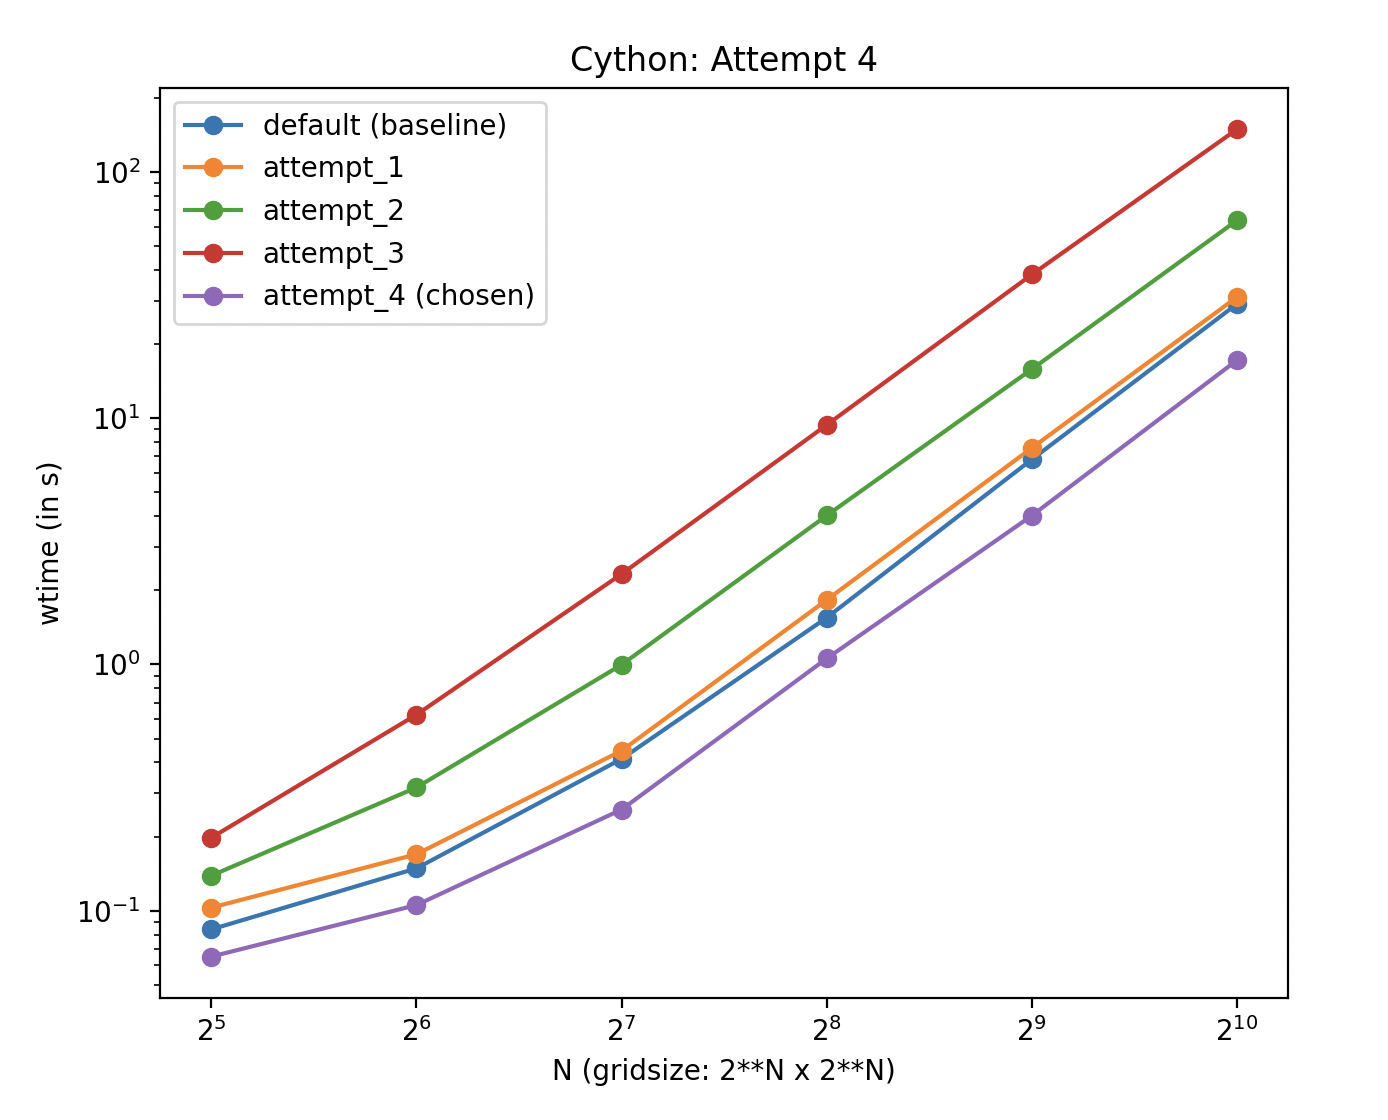
\includegraphics[width=0.7\textwidth]{images/cython/cython_attempt_4.png}
  \caption{Attempts 1-4 vs Baseline}
  \label{fig:cython_attempts}
\end{figure}

% \begin{figure}[h!]
 %   \begin{minipage}{0.45\textwidth}
 %       \centering
 %       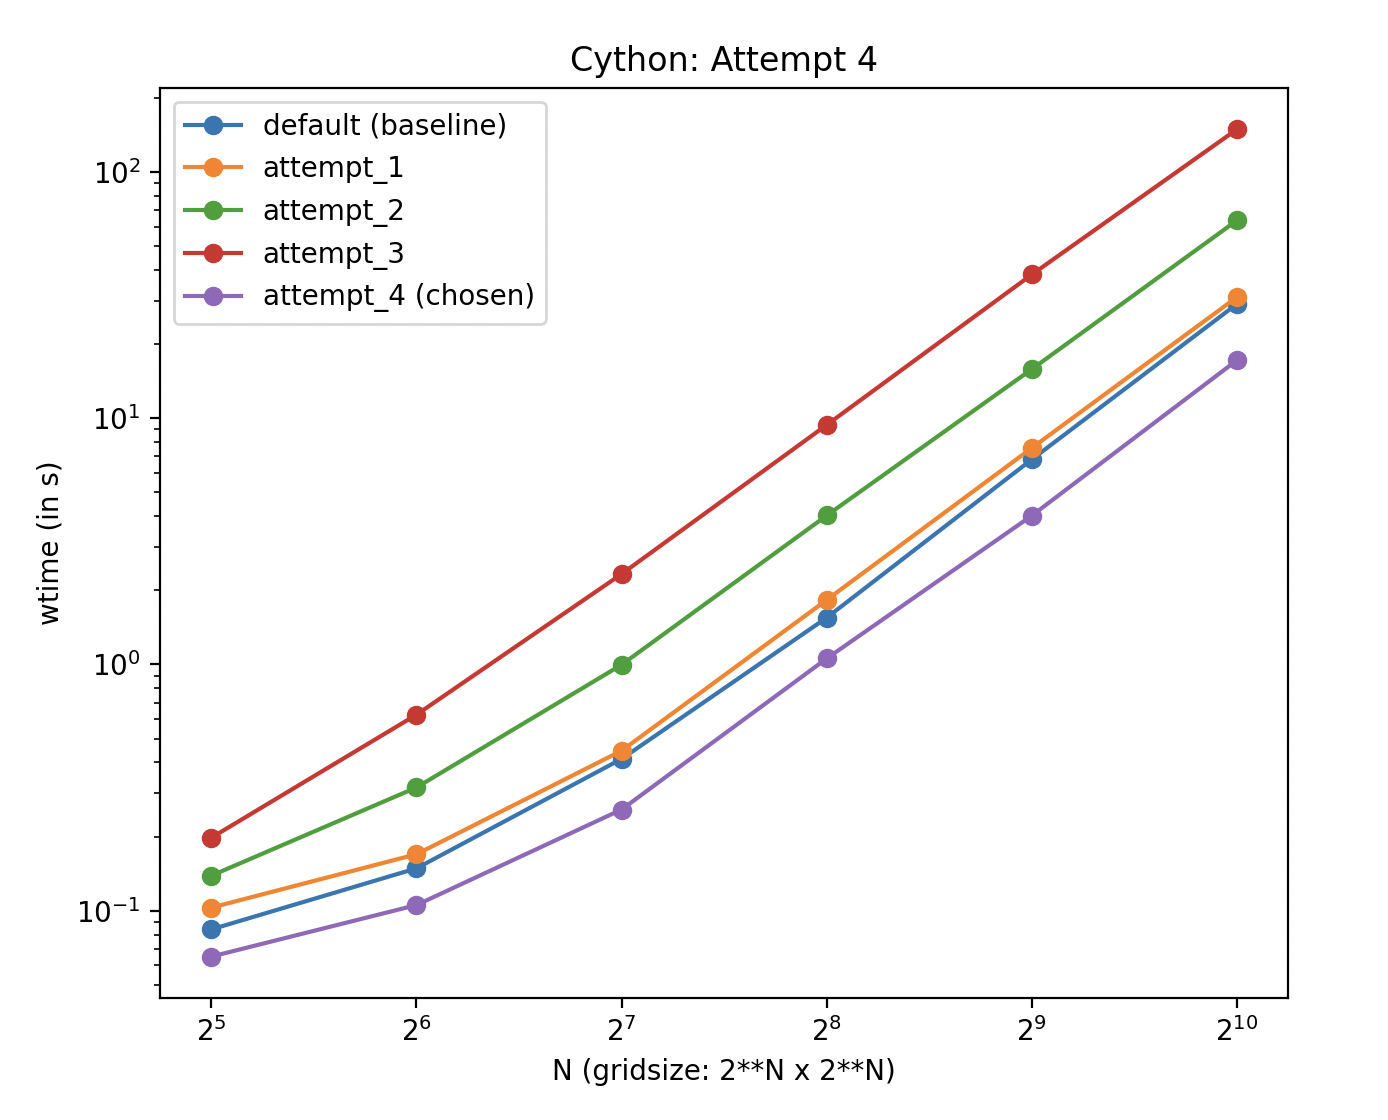
\includegraphics[width=\linewidth]{images/cython/cython_attempt_4.png}
%        \caption{Attempts 1-4 vs Baseline}
    %    \label{fig:cython_attempts}
  %  \end{minipage}
   % \hspace{0.1cm}
 %   \begin{minipage}{0.45\textwidth}
  %      \centering
  %      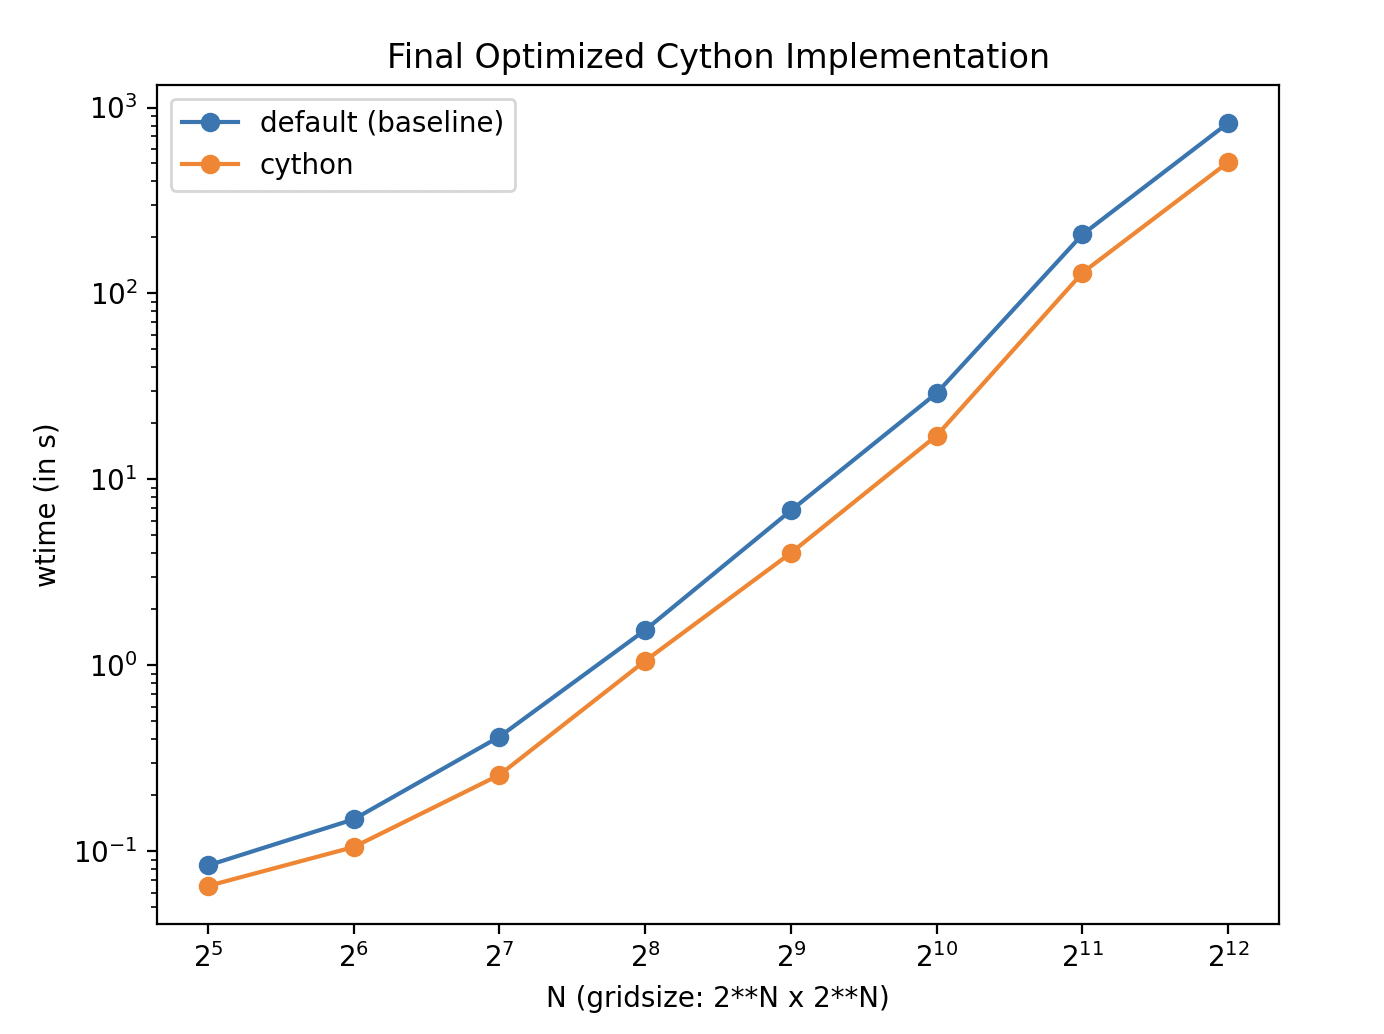
\includegraphics[width=\linewidth]{images/cython/cython_final_plot.png}
  %      \caption{Attempt 4 on Larger Grids}
 %   \end{minipage}
    
 %   \caption{Cython Optimizations}
% \end{figure}

\subsection{Attempt 3: Single \textbf{Python} Loop}
We observed that all the computations for the returned fluxes can be performend in an \textit{embarassingly parallel} manner: no cell of the retunred grids dependend on any other cell.
Thus, iterating over the input grids one cell at a time and computing the resulting fluxes would give us the same result as the vectorized version.
We implemented
\footnote{Code found \href{https://github.com/paulmyr/DD2358-HPC25/blob/master/10_project_rishi_paul/code/cython/finitevolume_cython_lib.pyx\#L287}{here} \textit{(getFlux)}.}
a \emph{single} nested loop in Python, where we compute each flux component one cell at a time.
We still use typed memoryviews.
We disabled some cython flags (such as \verb|boundscheck|, \verb|wraparound|) to help with speed.
The comparison of this attempt with the previous attempts and baseline can be seen in Figure \ref{fig:cython_attempts}. 

The performance was the worst out of all attempts.
This was suprising to us: we believed that Cython would be able to minimize the number of calls to the Python runtime because the nested loops involved only arithmetic operations on elements of typed memoryviews.
However, on examining the HTML file generated using the \verb|cython -a ...| command, we still observed heavy Python runtime calls for computations, particularly those that involved accessing elements of the typed memoryviews \footnote{can be seen in \hyperref[fig:cython_attempt_3_annotated]{Appendix}}.
The frequent callbacks to the Python runtime must have reduced the number of optimizations that Cython was able to make --- leading to worse performance.

\subsection{Attempt 4 (Chosen Optimization): Single \textbf{C} Loop}
We believed our intuition of using a single \verb|for-| loop was correct.
However Cython was not able to prevent the Python runtime interactions because of the reasons listed above.
Thus, we decided to reimplement\footnote{Code found \href{https://github.com/paulmyr/DD2358-HPC25/blob/master/10_project_rishi_paul/code/cython/finitevolume_cython_lib.pyx\#L359}{here} \emph{(getFluxRawC)}.} the core logic of the original \verb|getFlux| method in C ourselves.
The syntax and structure of the implementation was inspired by the example presnet in the Cython documentation (\href{https://docs.cython.org/en/latest/src/userguide/memoryviews.html\#pass-data-from-a-c-function-via-pointer}{link})
The C-implementation of the \verb|getFlux| loop-logic can be found in the \verb|flux.c| file \href{https://github.com/paulmyr/DD2358-HPC25/blob/master/10_project_rishi_paul/code/cython/flux.c}{link}.
The numpy arrays passed to the \verb|getFluxRawC| function appear to be in contiguous row-major (C) order, which makes the port of the python code to C easier.
We also have correctness tests in the \verb|flux_test.py| file (\href{https://github.com/paulmyr/DD2358-HPC25/blob/master/10_project_rishi_paul/code/cython/flux_test.py}{link}) to verify similarity between the default \verb|getFlux| and \verb|getFluxRawC|.
We still use typed memoryviews for the numpy arrays, along with disablement of some Cython flags. 


The runtime-comparison of this approach with the other attempts and baseline is present in Figure \ref{fig:cython_attempts}.
This is the best out of all approaches, and is \underline{\textbf{better than the baseline}} for all grid sizes.
We believe this highlights that our intuition of performing everything in one-loop was correct, along with our belief thatCython was unable to correctly optimize our implementation in Attempt-3.
In Figure \ref{fig:cython_final_plot}, we see that the performance of this approach remains better than the baseline for grid sizes 2048 and 4096.
The bar graphs in Figure \ref{fig:cython_final_bar} highlights the performance difference of this Cython optimization over the baseline.
This was chosen as our Cython optimization of the original problem, and the code used for generating the plots and running the simulation is in the \verb|finitevolume_cython.py| file (\href{https://github.com/paulmyr/DD2358-HPC25/blob/master/10_project_rishi_paul/code/cython/finitevolume_cython.py}{link})
\begin{figure}[h!]
   \begin{minipage}{0.5\textwidth}
       \centering
       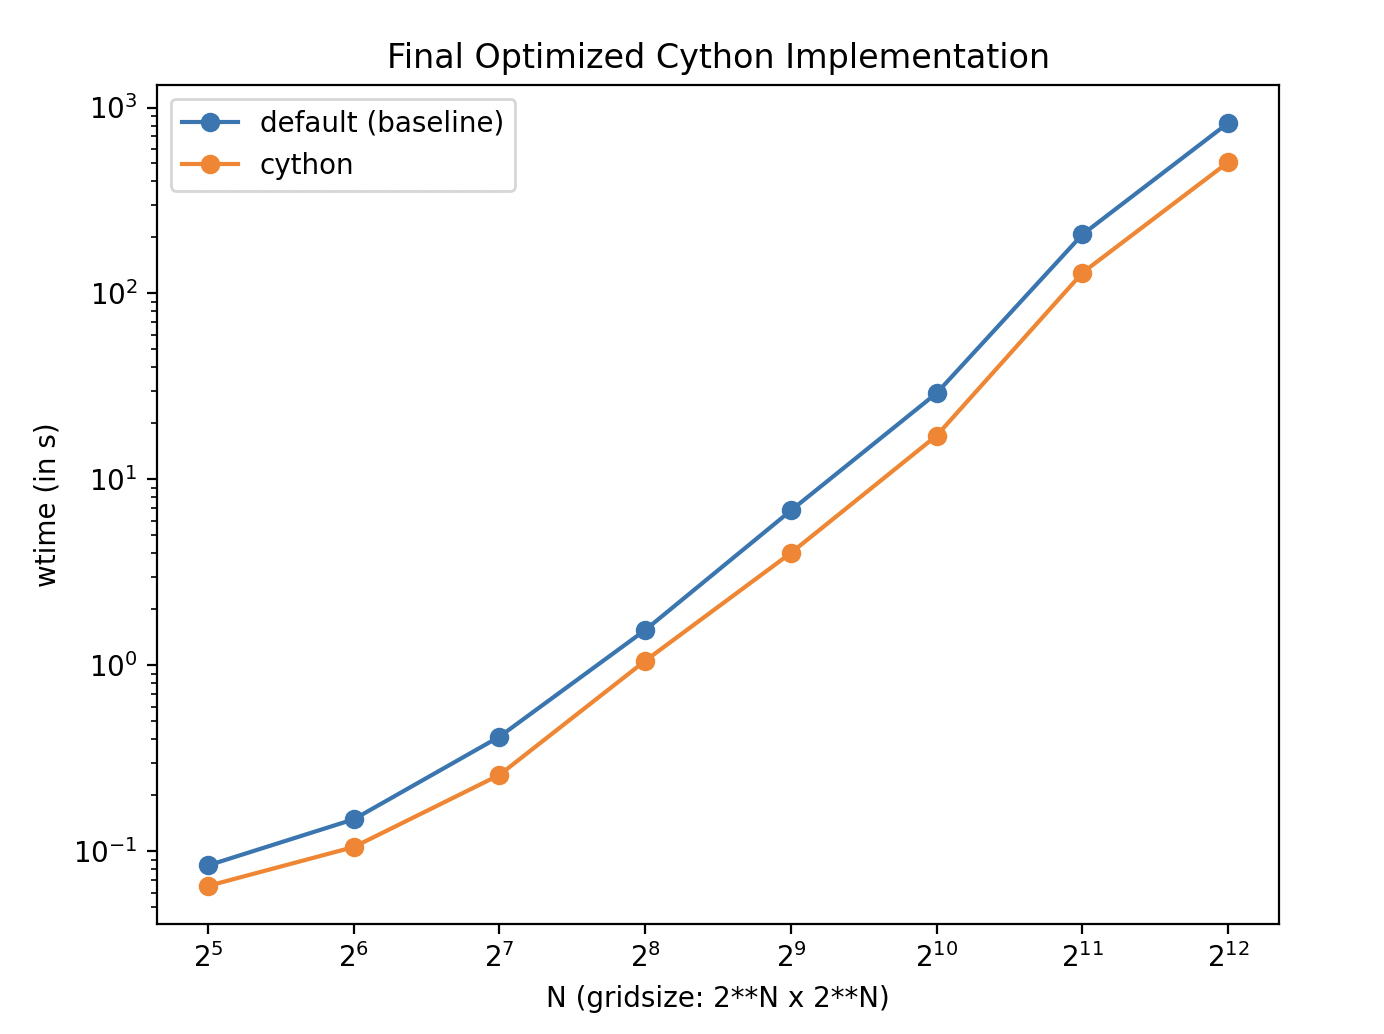
\includegraphics[width=\linewidth]{images/cython/cython_final_plot.png}
      \caption{Line Plot}
       \label{fig:cython_final_plot}
   \end{minipage}
   \hspace{0.1cm}
   \begin{minipage}{0.5\textwidth}
       \centering
       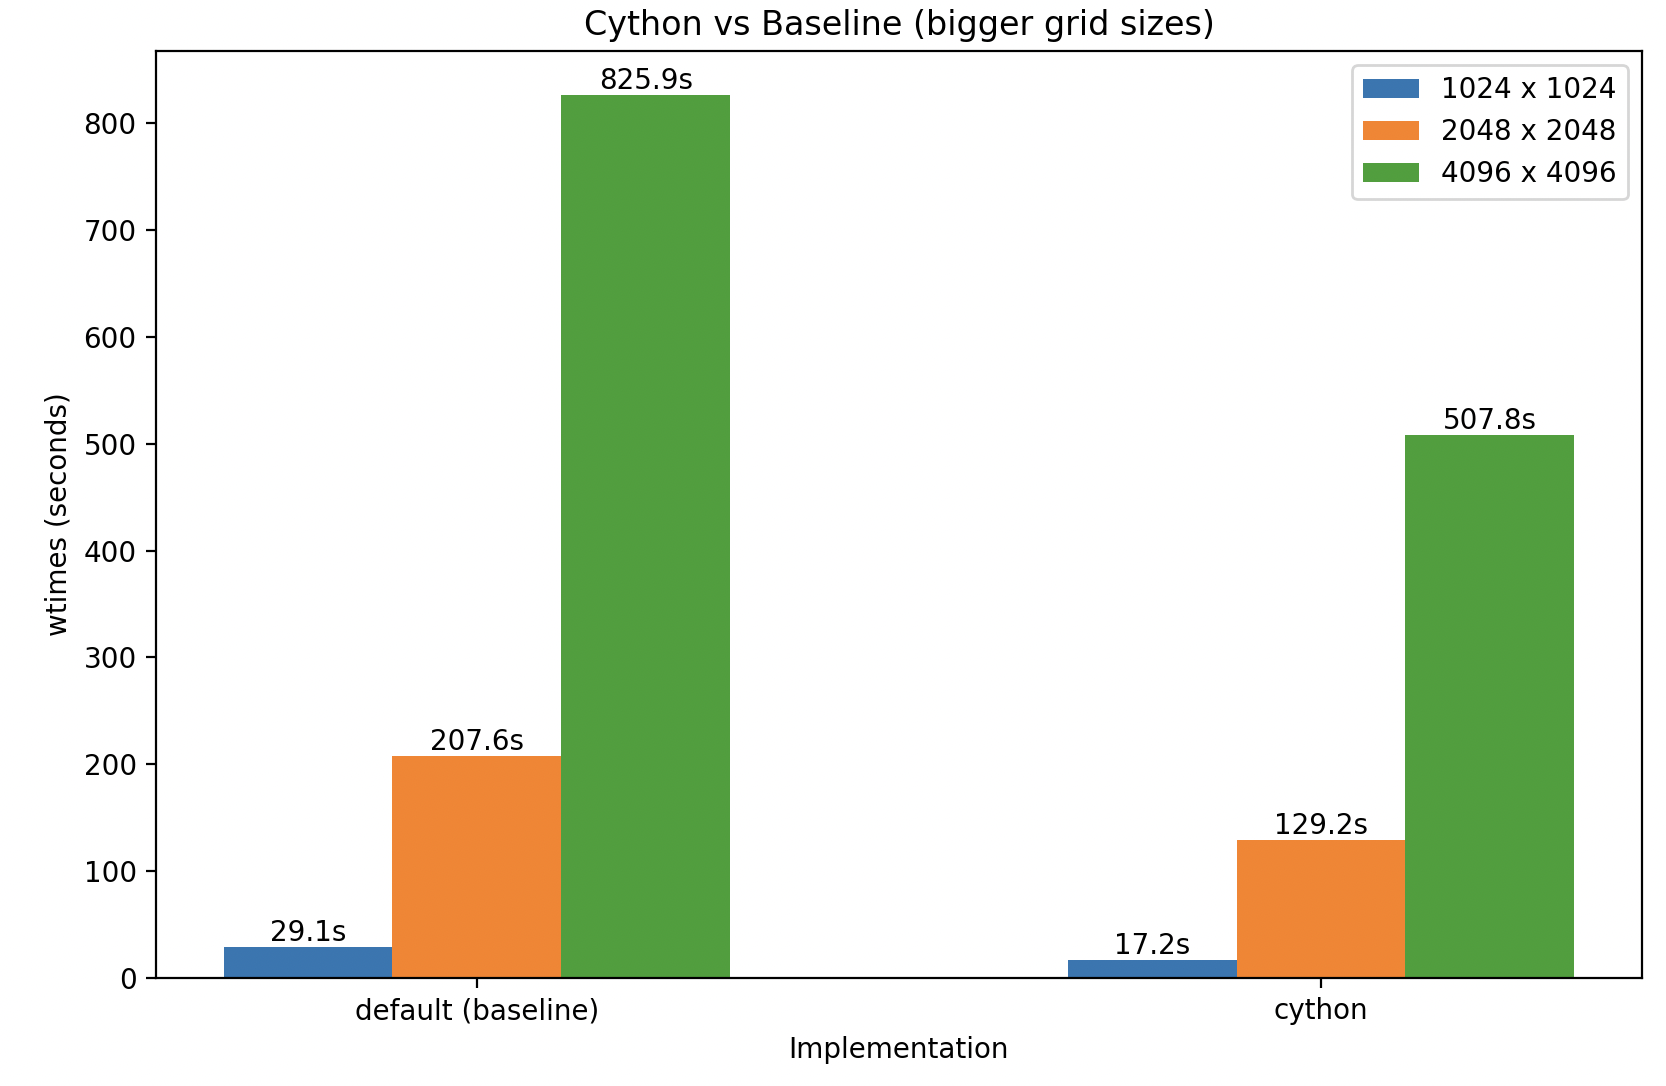
\includegraphics[width=\linewidth]{images/cython/cython_final_bar.png}
      \caption{Bar Graph}
      \label{fig:cython_final_bar}
  \end{minipage}
  \caption{Cython Attempt 4 vs Baseline}
\end{figure}

%\begin{figure}[h]
%  \centering
%  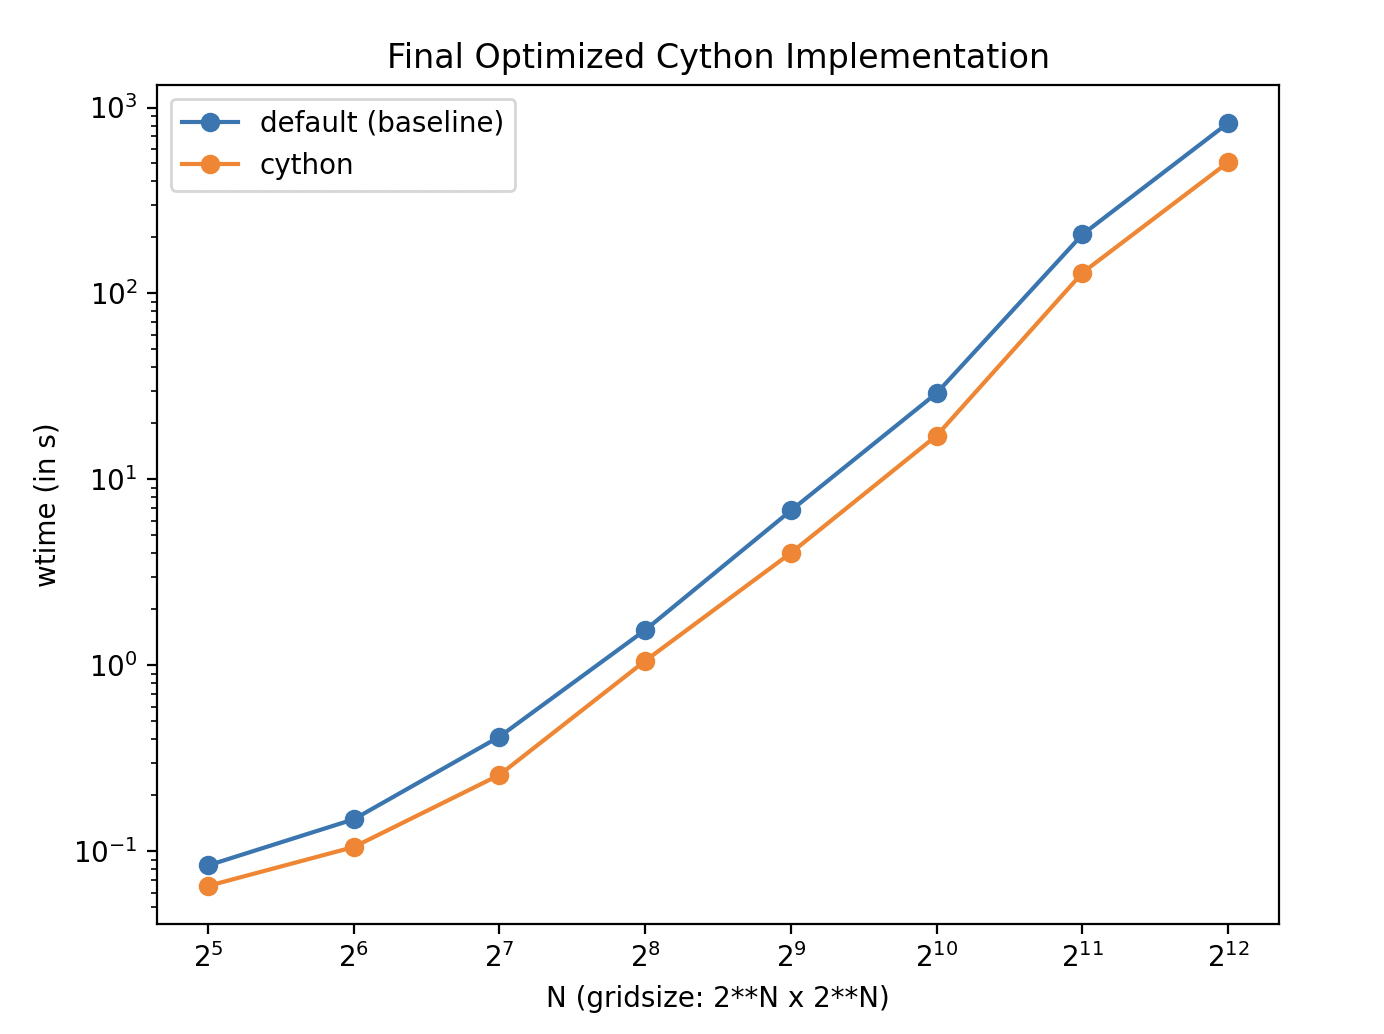
\includegraphics[width=0.7\textwidth]{images/cython/cython_final_plot.png}
%  \caption{Attempt 4 on Larger Grids}
%  \label{fig:cython_final_plot}
%\end{figure}

\section{Optimizations using Pytorch}
The original implementation makes heavy use of numpy functionalities.
All data is stored as numpy arrays that are incrementally updated using the computed fluxes.
This provides an easy approach to move the computations on a GPU using pytorch.
Pytorch's computations are run using tensors --- an immutable datatype that shares resemblence with numpy arrays.
A big difference however is that tensor operations are supported to be computed using accelerators.
Due to the fact that pytorch mirrors numpys interface, we simply need to convert said numpy arrays to pytorch tensors
and tell pytorch to perform the computations using GPU compatible hardware.
\todo[inline]{insert figure of GPU runtimes}

To compare the performance on a wider range of grid sizes, we chose to limit the simulation to a fixed number time steps.
As one can see\todo{describe figure before referencing it} in the results of figure, making use of accelerators *greatly* improves the overall runtime for larger grid sizes.
As noted above \todo{insert ref to figure}, for finer grids this means we simulate less time in total.
\todo[inline]{For the pytorch mps runtime, describe that it was obtained on m1 pro}

\section{Optimizations using Dask}
We had 2 attempts at optimzing the baseline using Dask.
The code for this section is present in the \verb|dask/| directory of the repository.
All runtimes presented in this section timed the simulation for 256 iterations using our different optimization attempts, and were obtained on a 2021 M1 Macbook Pro (16').
The \underline{line plots} of runtimes are \underline{logarithmic} (base 10).
We also have tests in the \verb|test_dask_rho.py| file, which check that the final \verb|rho| visualized on the grid is similar for the chosen Dask optimization and the baseline.
For all dask runs, the default scheduler settings were used, which on the environment stated above, gave us \underline{5 workers, 2 threads per worker}.

The fact that each iteration of the simulation dependend on the outputs of the previous iteration, coming up with Dask optimizations that delayed the call to \verb|compute()| till the last possible moment (preferably outside the loop), was difficult.
Particularly, the termination condition of the original code dependend on the time parameter \verb|t|, which was updated in every iteration based on the value of \verb|dt| that was computed inside the loop.
Thus, the 2 optimizations we tried respect this starting structure of the code, and consequently \verb|compute()| is called \underline{in each iteration}.
While not a best pracitce, we were still able to obtain promising results from our second optimization.

\begin{figure}[h]
  \centering
  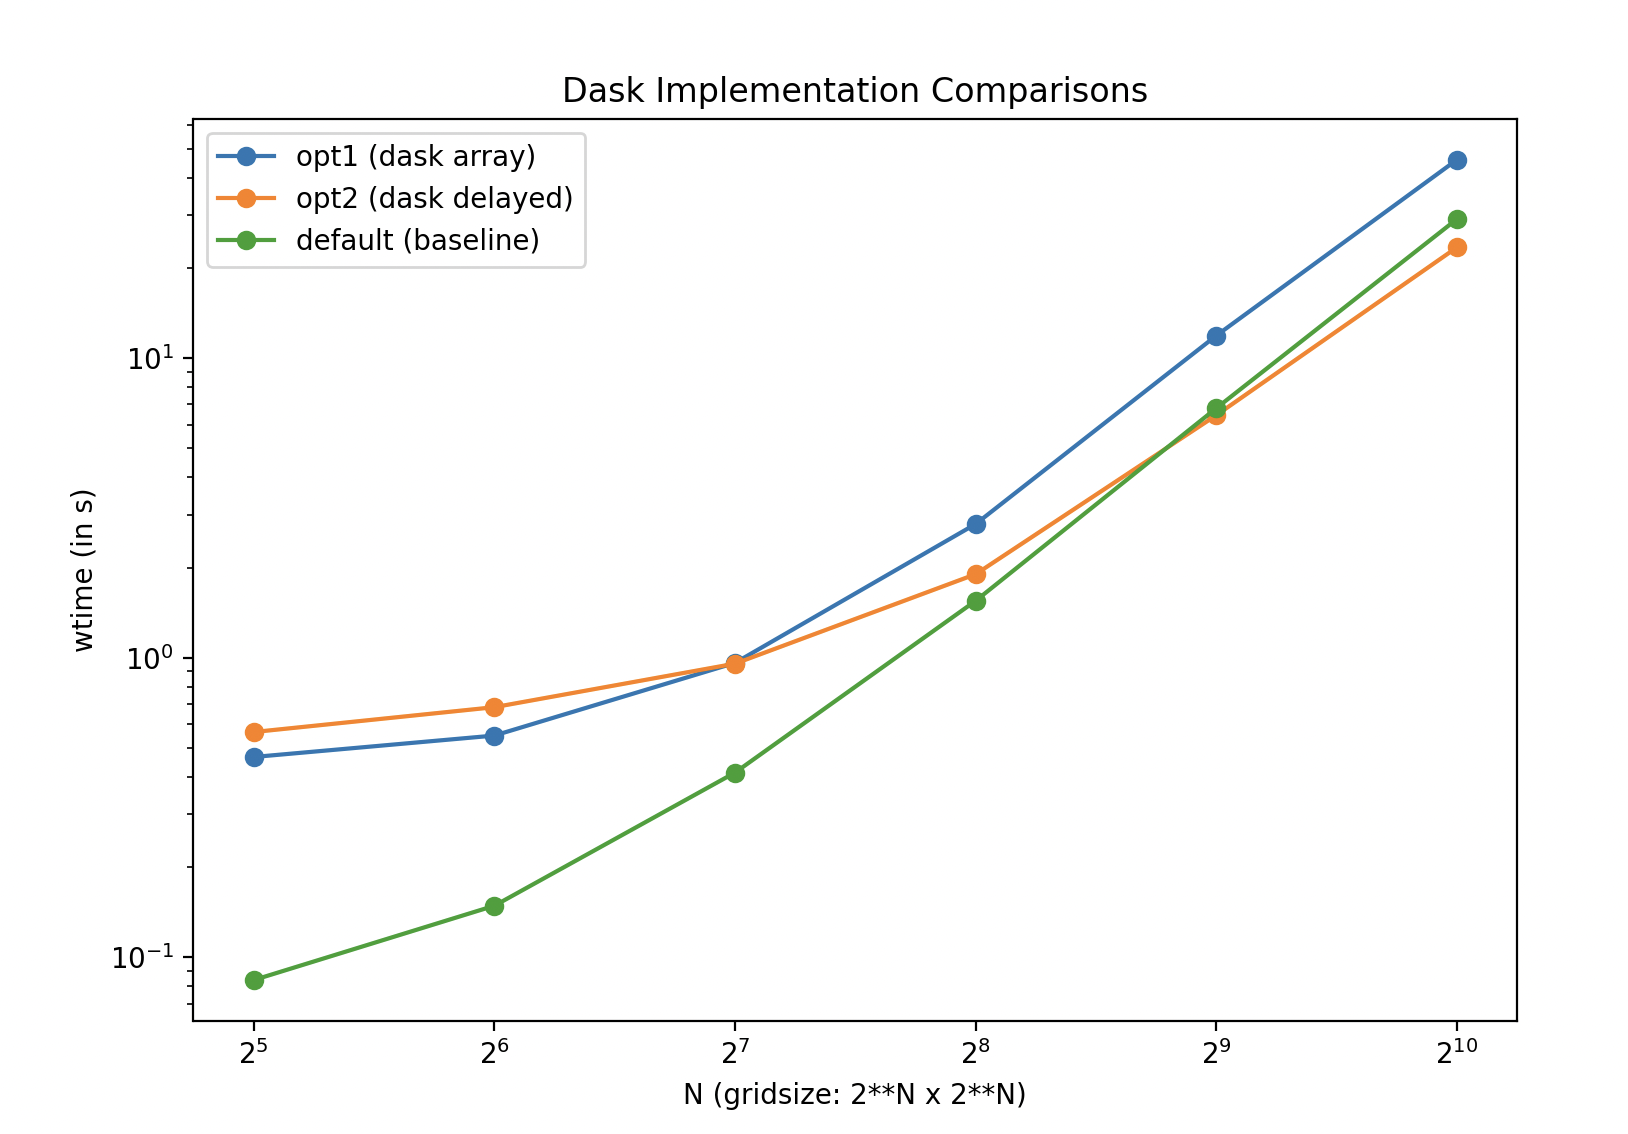
\includegraphics[width=0.7\textwidth]{images/dask/dask_comparison.png}
  \caption{Dask Attempts 1-2 vs Baseline}
  \label{fig:dask_attempts}
\end{figure}

\subsection{Attempt 1: Dask Arrays}
The code for this attempt can be found in the \verb|finitevolume_dask_opt1.py| file (\href{https://github.com/paulmyr/DD2358-HPC25/blob/master/10_project_rishi_paul/code/dask/finitevolume_dask_opt1.py}{link}).
As noted earlier, \verb|getFlux| was the bottleneck for the baseline simulation, and it was \textit{embarassingly parallelizable} (no cell computation dependend on any other cell).
So, we used \verb|map_blocks| from \verb|dask.arrays| on the \verb|getFlux| for the \verb|getFlux| method.
We only used this for the compuatation of the fluxes in \verb|x-| direction first, hoping to extend it to \verb|y-| direction if the performance was good.
We created dask arrays for the input to \verb|getFlux| in each iteration.
We then called \verb|compute()| on the value returned by \verb|map_blocks| to obtain the fluxes in \verb|x-| direction in each loop iteration.
The task-stream visualizations were done while running the experiment on a grid size of 128 till 2 seconds of \underline{simulated time}.
\begin{figure}[h!]
   \begin{minipage}{0.5\textwidth}
       \centering
       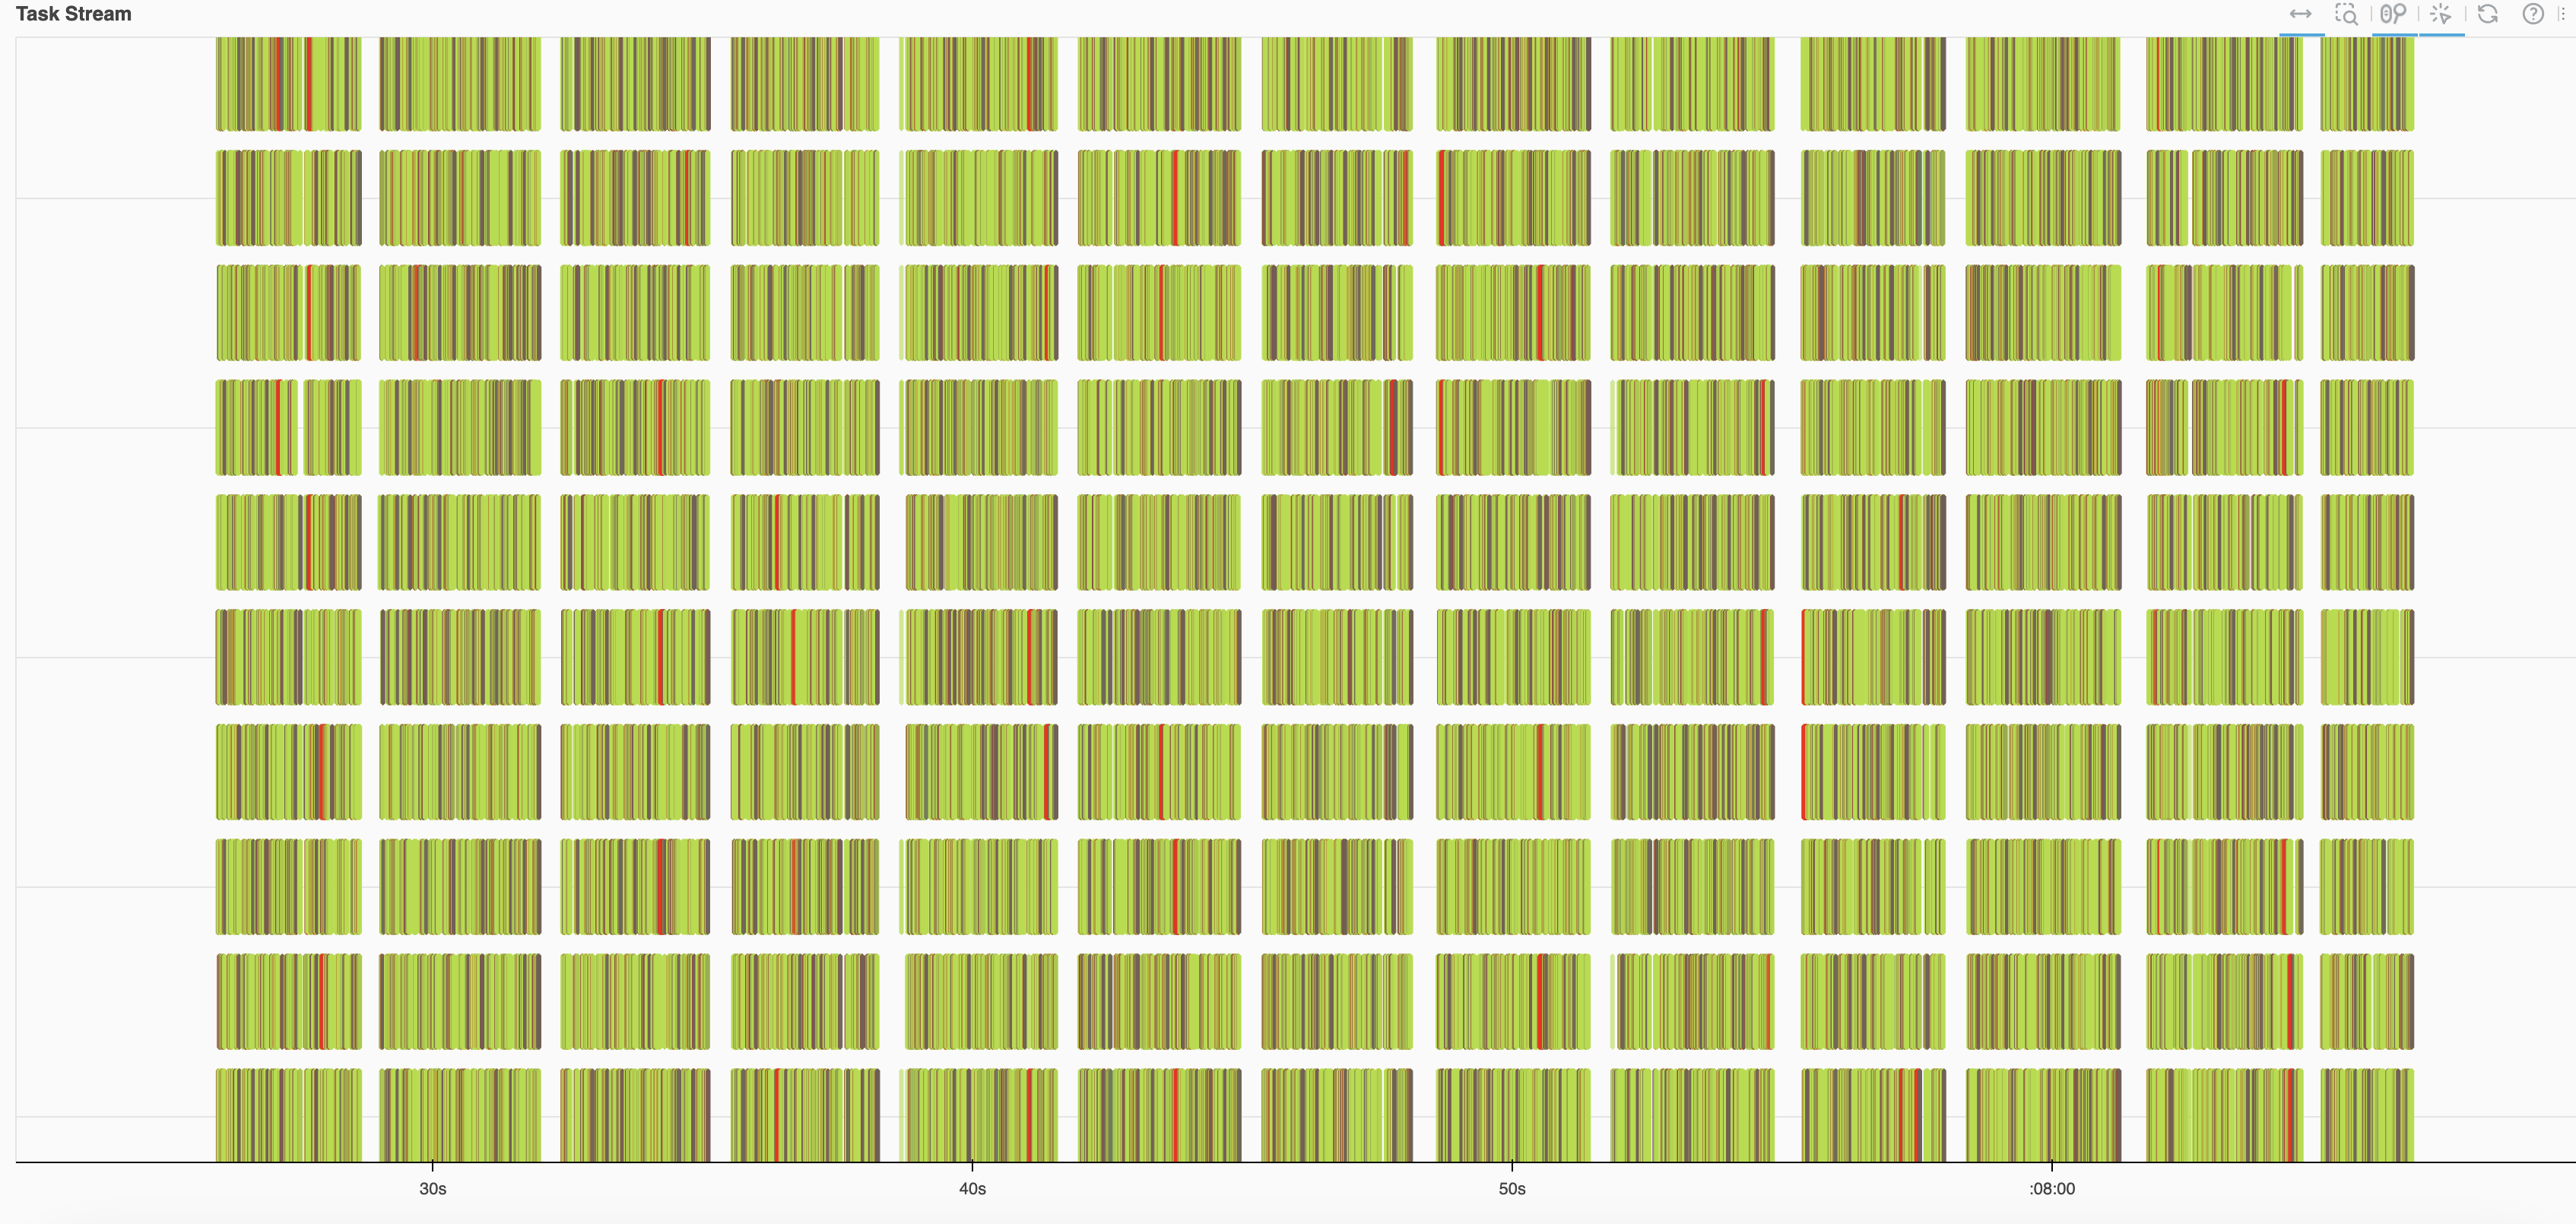
\includegraphics[width=\linewidth]{images/dask/dask_opt1_n_by_8.png}
      \caption{Work Stream (64 chunks)}
       \label{fig:dask_opt1_stream_64}
   \end{minipage}
   \hspace{0.1cm}
   \begin{minipage}{0.5\textwidth}
       \centering
       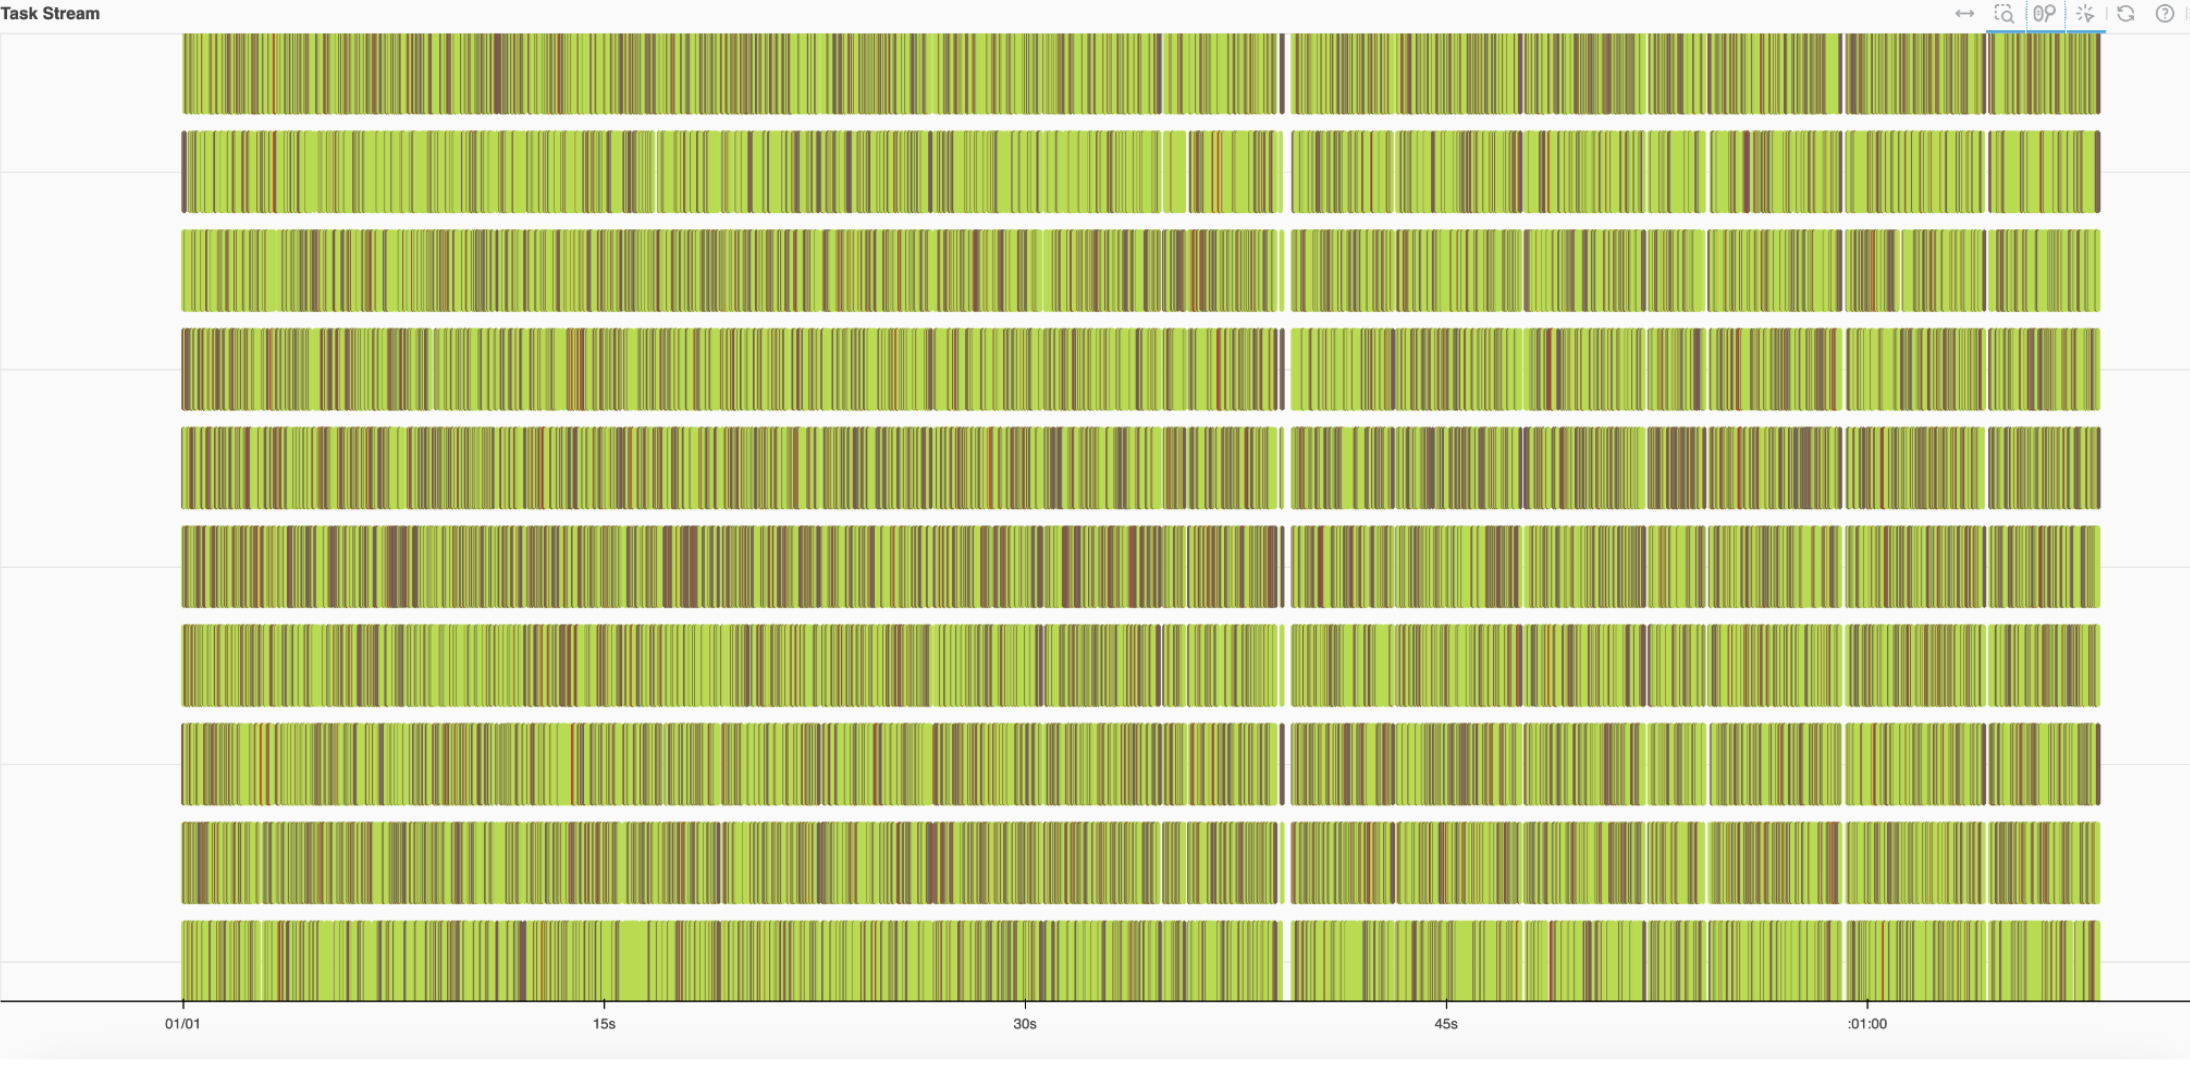
\includegraphics[width=\linewidth]{images/dask/dask_opt1_n_by_2.png}
      \caption{Work Stream (4 chunks)}
      \label{fig:dask_opt1_stream_4}
  \end{minipage}
  \caption{Work Stream for Dask Attempt 1}
  \label{fig:dask_opt1_stream}
\end{figure}
We varied the chunk sizes of the dask arrays to see what impact they have on the runtime.
A plot of this can be seen in the \hyperref[fig:dask_opt1_chunk_size]{Appendix}.
In Figure \ref{fig:dask_attempts}, we present only the plot for the best chunk-size (which was 1).
In summary, the performance decreased with an increase in chunk-sizes.

The performance of this implementation \underline{always seems to be worse than the baseline}.
We believe several factor could have contributed to this.
Firstly, there is some overhead involved in dask having to create the dask arrays with the correct chunk sizes, allocating them to the workers, setting up the scheduler, etc.
This overhead can be present in the form of communication between workers.
This was observed on the task-stream for the computation on the Dask Dashboard.
The red/dark-red observed in the task stream in Figure \ref{fig:dask_opt1_stream} indicates a lot of transfer between workers, as documented \href{https://docs.dask.org/en/stable/dashboard.html\#task-stream}{here}.
This was also present when we had fewer chunks than cores/workers (Figure \ref{fig:dask_opt1_stream_4}).
Additionally, the call to compute in each loop iteration would also lead to a slowdown.

We thought of some ideas to address some of our concerns here (such as trying to delay \verb|compute| for everythinf except \verb|dt|).
However, our experience with Assignment 4's Bonus lead us to believe that even with fewer \verb|compute()| calls, the performance of dask-arrays in a single-machine environment would likely still be worse than the baseline (because of the set-up overhead discussed above).
Thus, before doing this, we tried a different approach: \verb|dask delayed|.

\subsection{Attempt 2 (Chosen Optimization): Dask Delayed}
This code can be found in the file \verb|finitevolume_dask_opt2.py| (\href{https://github.com/paulmyr/DD2358-HPC25/blob/master/10_project_rishi_paul/code/dask/finitevolume_dask_opt1.py}{link}) Instead of focusing only on the parallelizability of \verb|getFlux|, we observed that there were several calls ot helper functions that were independent of each other.
For instance, all calls to \verb|getGradient| in the simulation loop were independent of each other.
So, we looked at the \textit{bigger picture} and decided to use dask-delayed to store the delayed tasks for each helper function in an array, and then calling \verb|dask.compute()| for each element of the task array.
An example of this approach can be seen here (\href{https://github.com/paulmyr/DD2358-HPC25/blob/master/10_project_rishi_paul/code/dask/finitevolume_dask_opt2.py\#L273}{link}).
Each such helper function was tagged the \verb|@delayed| decorator.

\begin{figure}[h]
  \centering
  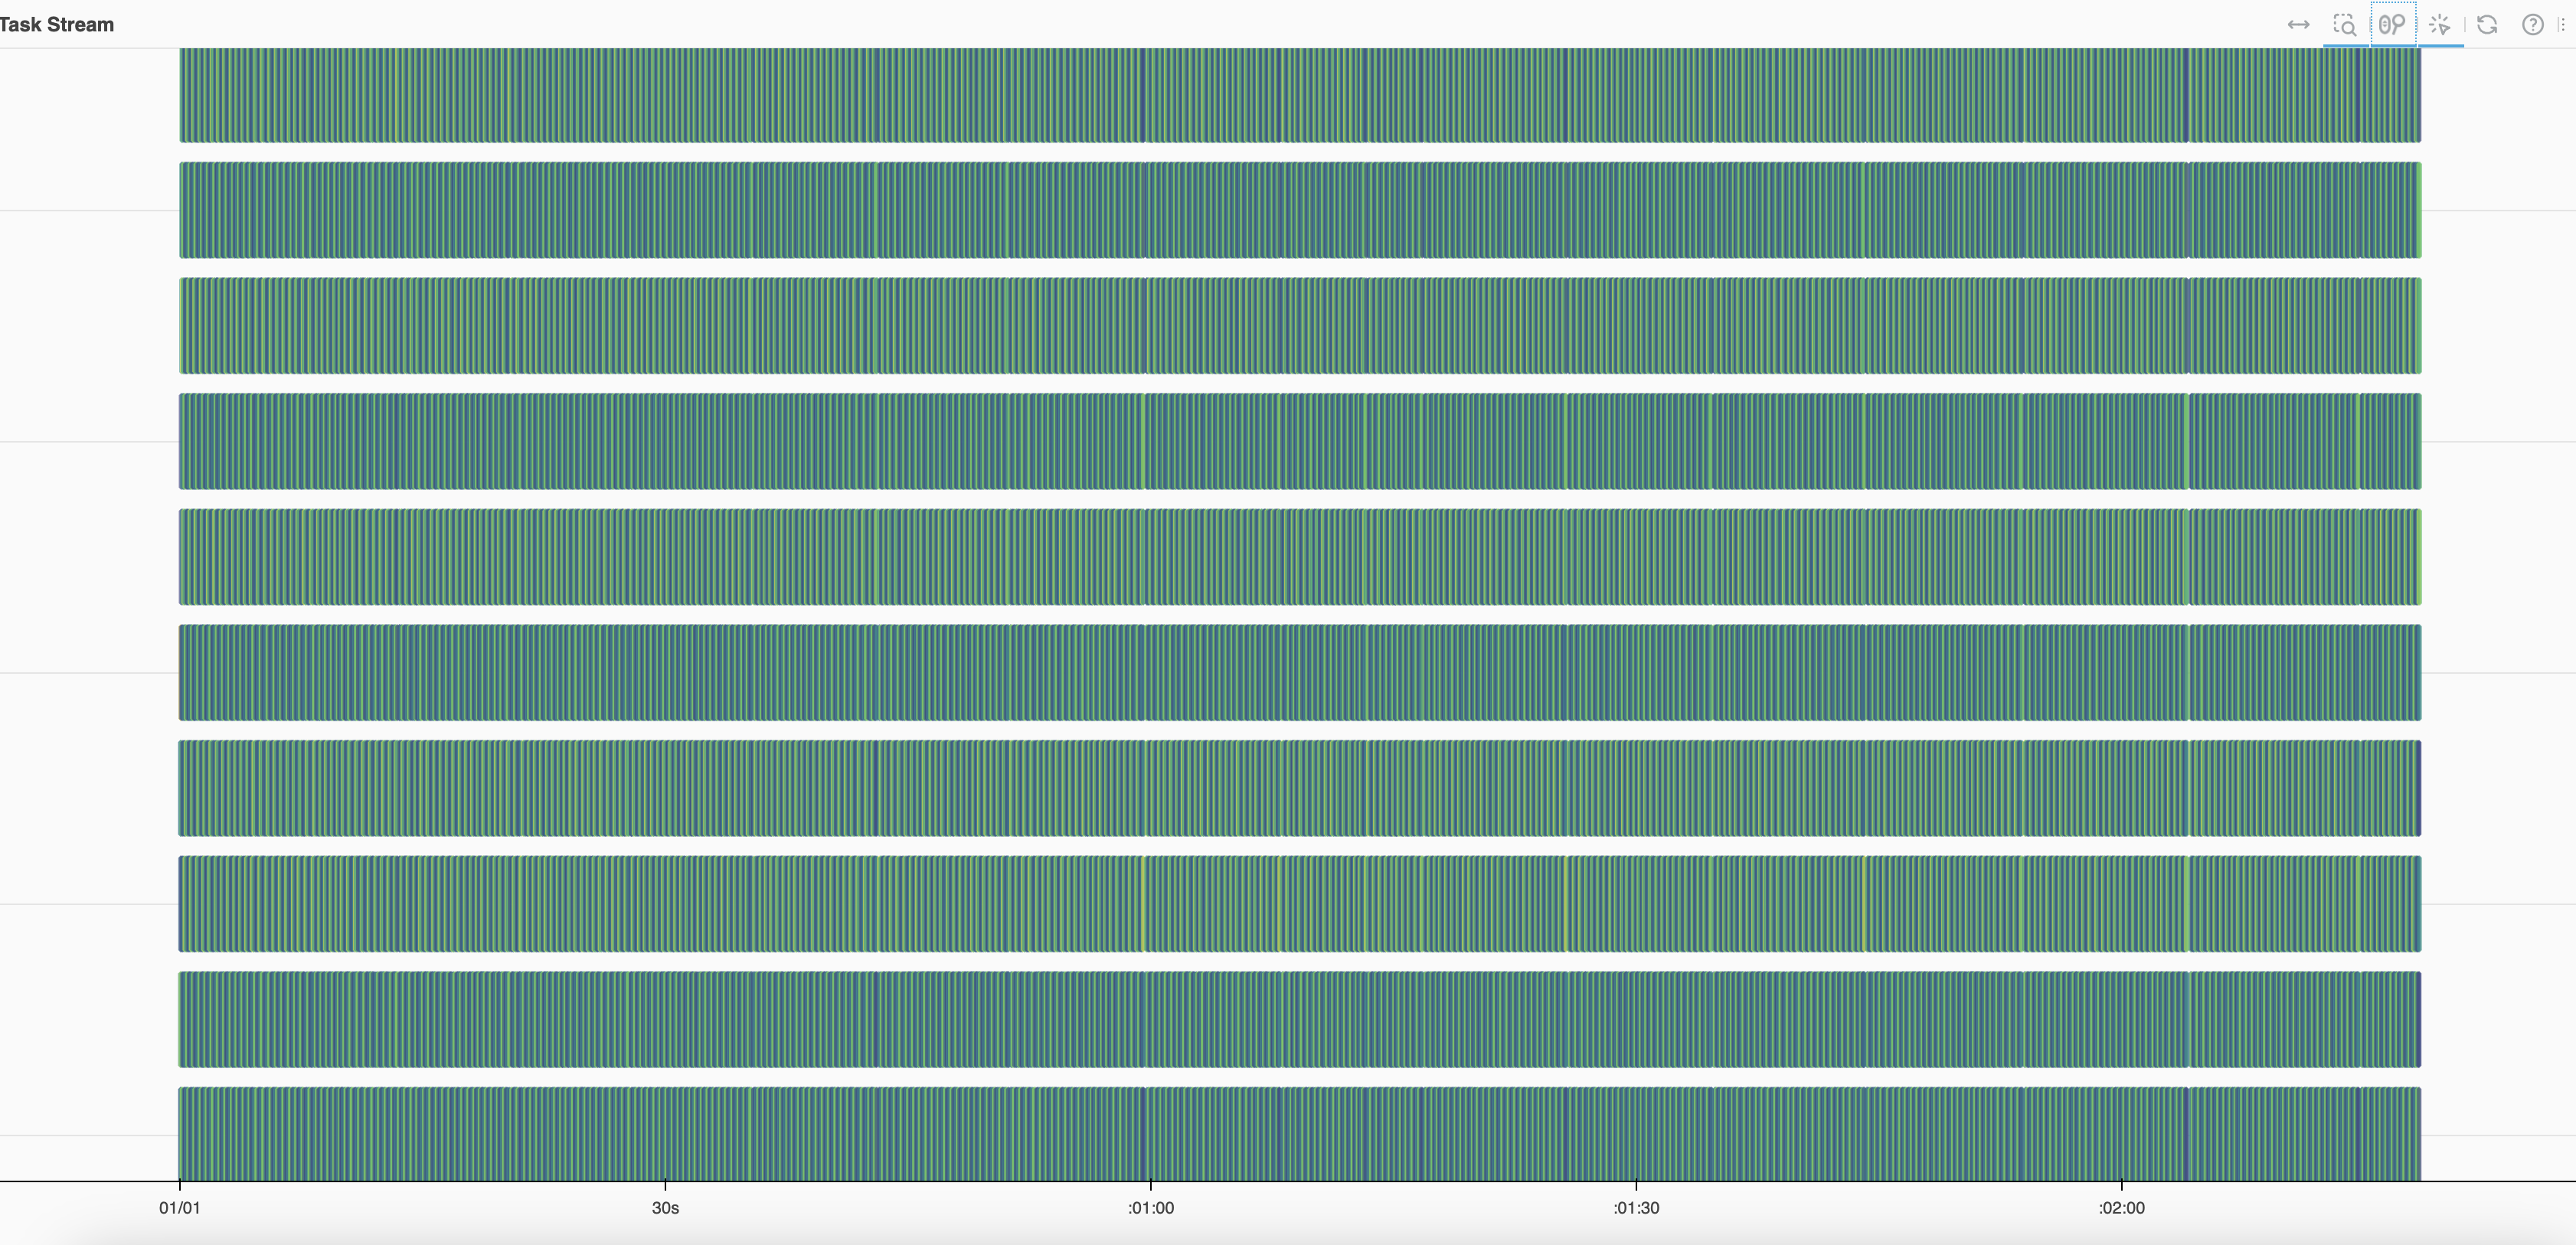
\includegraphics[width=0.7\textwidth]{images/dask/dask_opt2.png}
  \caption{Task Stream for Dask-Delayed Optimization}
  \label{fig:dask_opt2_stream}
\end{figure}

The performance of this implementation with Attempt-1 (dask-arrays) and baseline can be seen in Figure \ref{fig:dask_attempts}.
We see that initially for very small grids, this attempt performs the worst.
This could be because of the increased number of \verb|compute()| calls for each independent helper-function, which requires all parallel calls to complete before progressing.
This could be overkill for small grids.
\textit{However}, as the grid sizes increase, this attempt comes out on top. This indicates to us that as the grid-size increases, the sheer number of computations to be performed \underline{outweighs} the cost of the multiple \verb|compute()| calls (and other overhead required by dask-delayed): leading to a better performance when doing the computations in parallel for grid sizes 512 and 1024 (and likely even bigger grids) compared to the baseline.
The improved performance compared to Attempt-1 could be explained by almost no interaction required between workers, as can be seen by the absence of red in the task-stream graph in Figure \ref{fig:dask_opt2_stream}.
This was our chosen Dask optimization.

 \begin{figure}[h!]
    \begin{minipage}{0.5\textwidth}
        \centering
        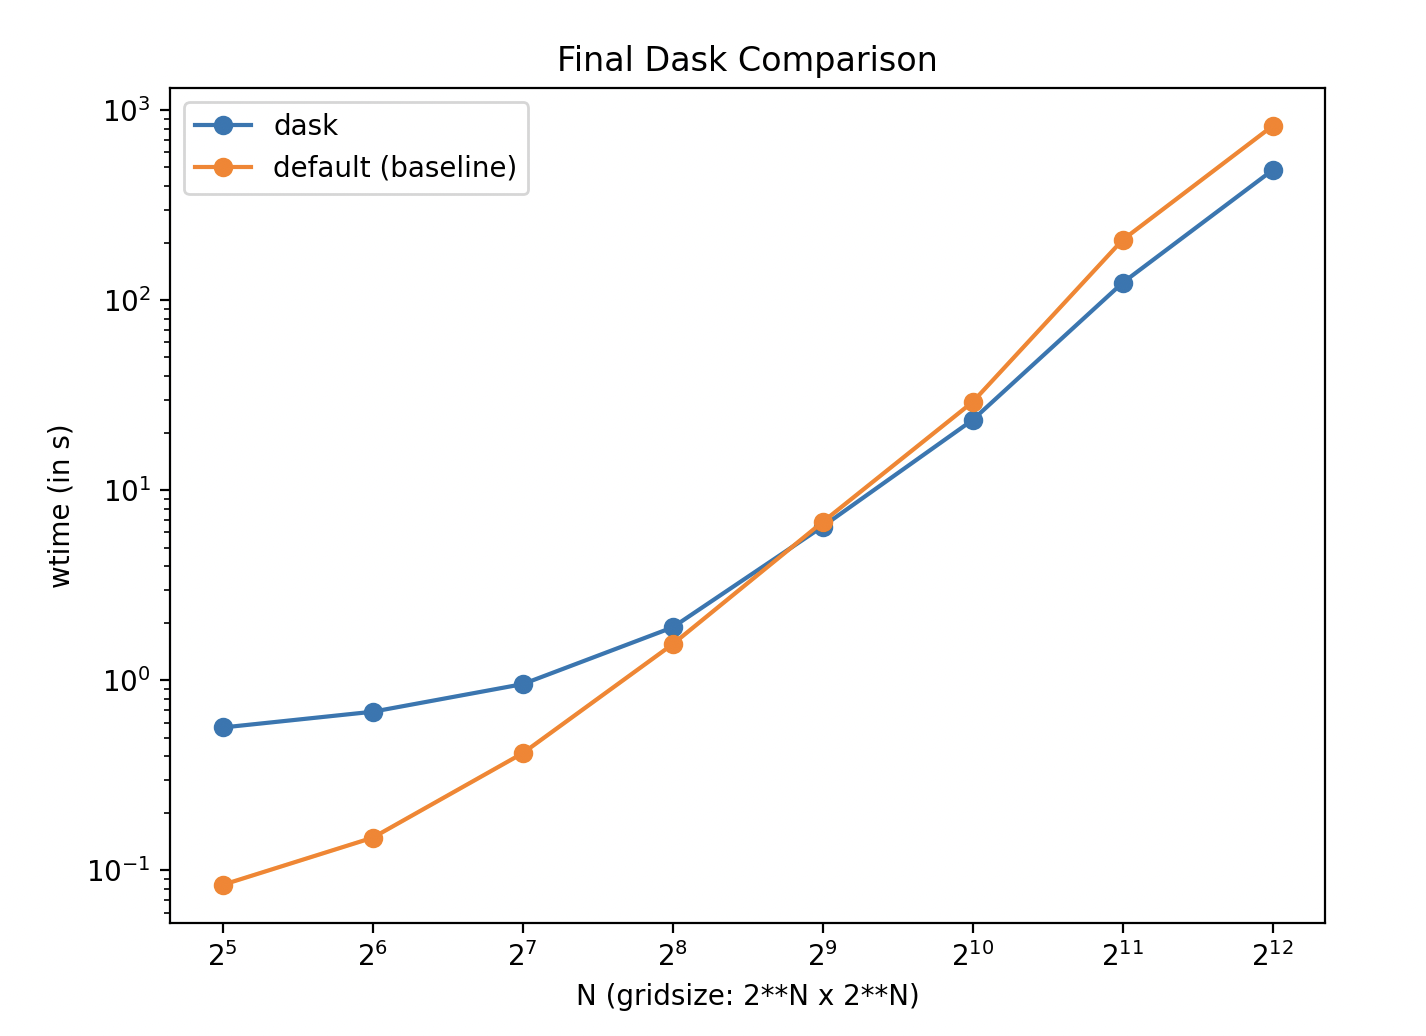
\includegraphics[width=\linewidth]{images/dask/dask_final_plot.png}
       \caption{Line Plot}
        \label{fig:dask_final_plot}
    \end{minipage}
    \hspace{0.1cm}
    \begin{minipage}{0.5\textwidth}
        \centering
        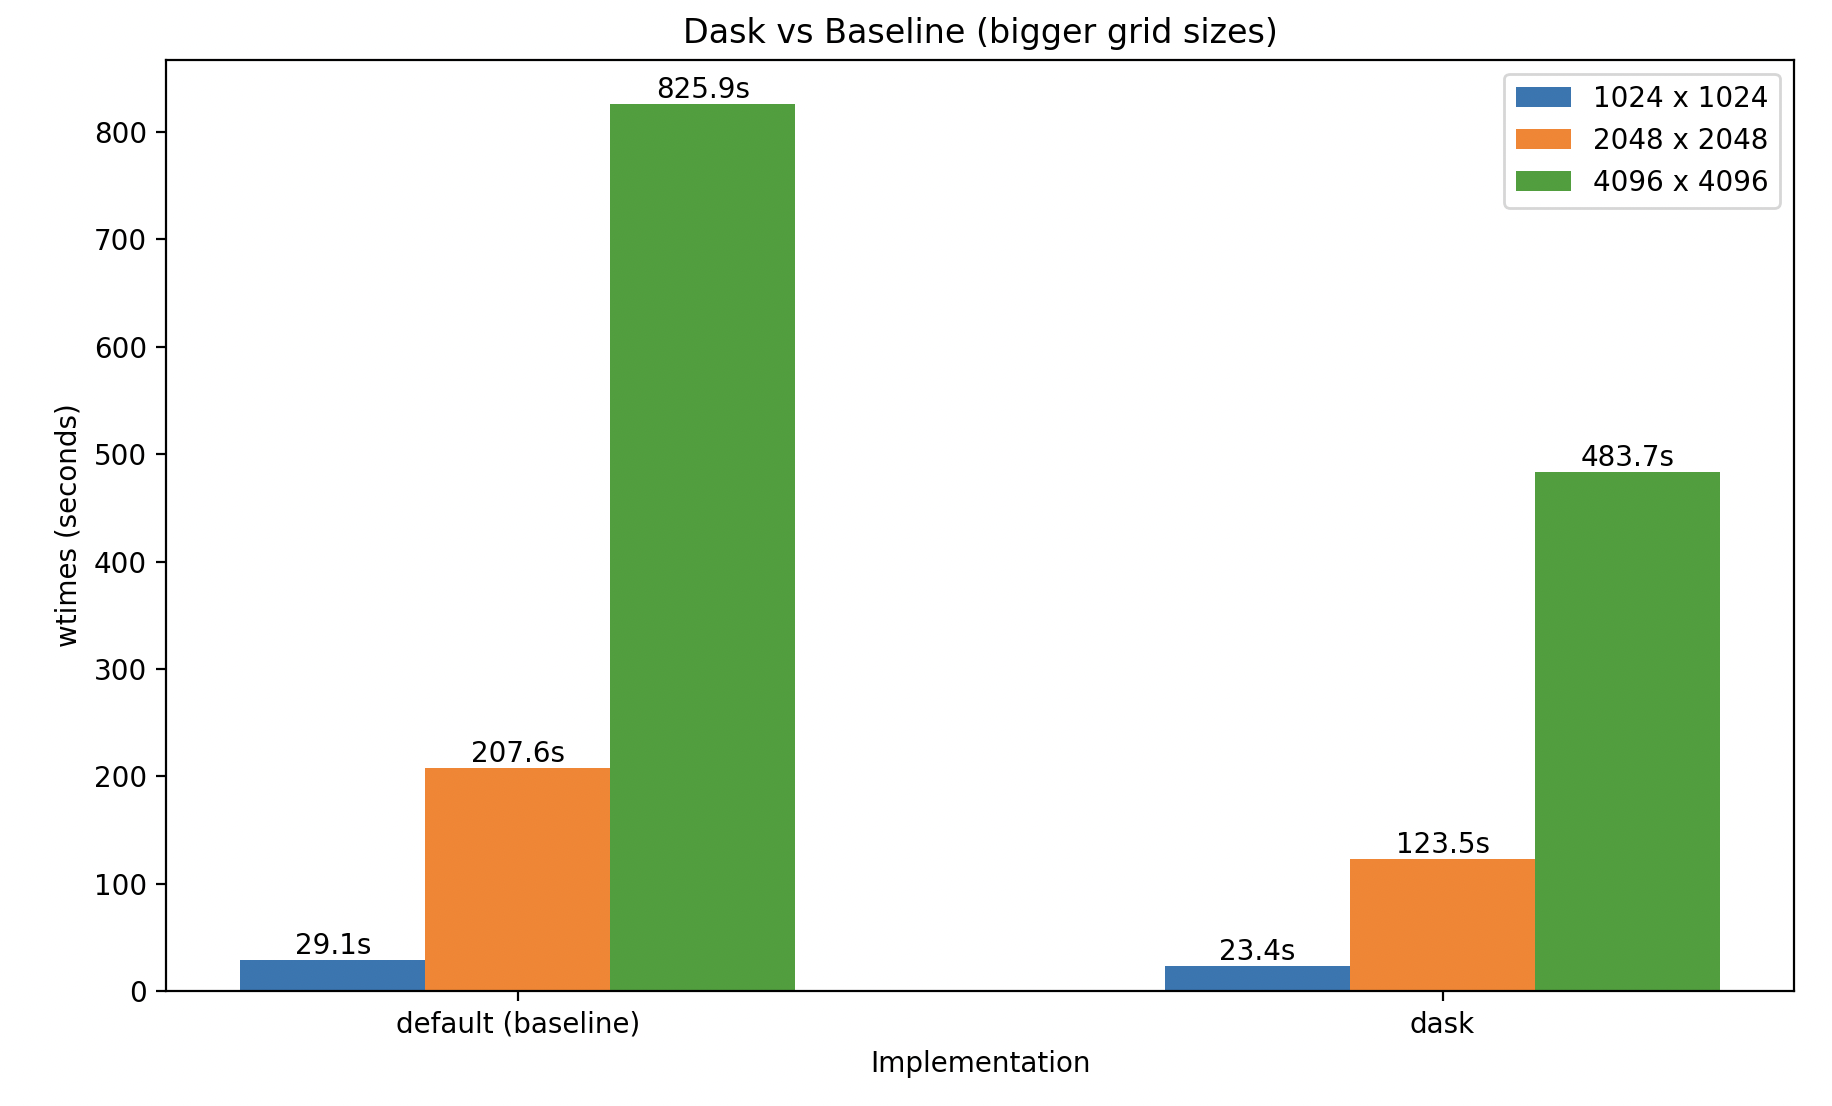
\includegraphics[width=\linewidth]{images/dask/dask_final_bar.png}
       \caption{Bar Graph}
       \label{fig:dask_final_bar}
   \end{minipage}
   \caption{Dask Attempt 2 vs Baseline}
 \end{figure}

 In Figure \ref{fig:dask_final_plot}, we see that the performance of this optimization remains better than the baseline for larger grids, as we hypothesized.
 Figure \ref{fig:dask_final_bar} highlights the time-difference that might be lost in the log-scale based line plot.

\section{Bonus Optimization: Cython + Dask}
We observed that for the 2 largest grid sizes (2048 and 4096), our Cython optimization performed \textbf{worse} than our Dask optimization.
To us, this indicated that any performance advantage obtained from performing the time-consuming \verb|getFlux| operations in C was lost when it came to the sheer number of operations to be performed, thus giving our parallel Dask optimization an advantage.

As a bonus, we decided to combine the two: we performed the \verb|getFluxRawC| computation (our Cython optimization) in parallel (using our Dask-Delayed optimization).
The code for this can be found in the \verb|finitevolume_cython_dask.py| file (\href{https://github.com/paulmyr/DD2358-HPC25/blob/master/10_project_rishi_paul/code/cython/finitevolume_cython_dask.py}{link}), particularly \href{https://github.com/paulmyr/DD2358-HPC25/blob/master/10_project_rishi_paul/code/cython/finitevolume_cython_dask.py\#L305}{this} line.

\begin{figure}[h!]
   \begin{minipage}{0.5\textwidth}
       \centering
       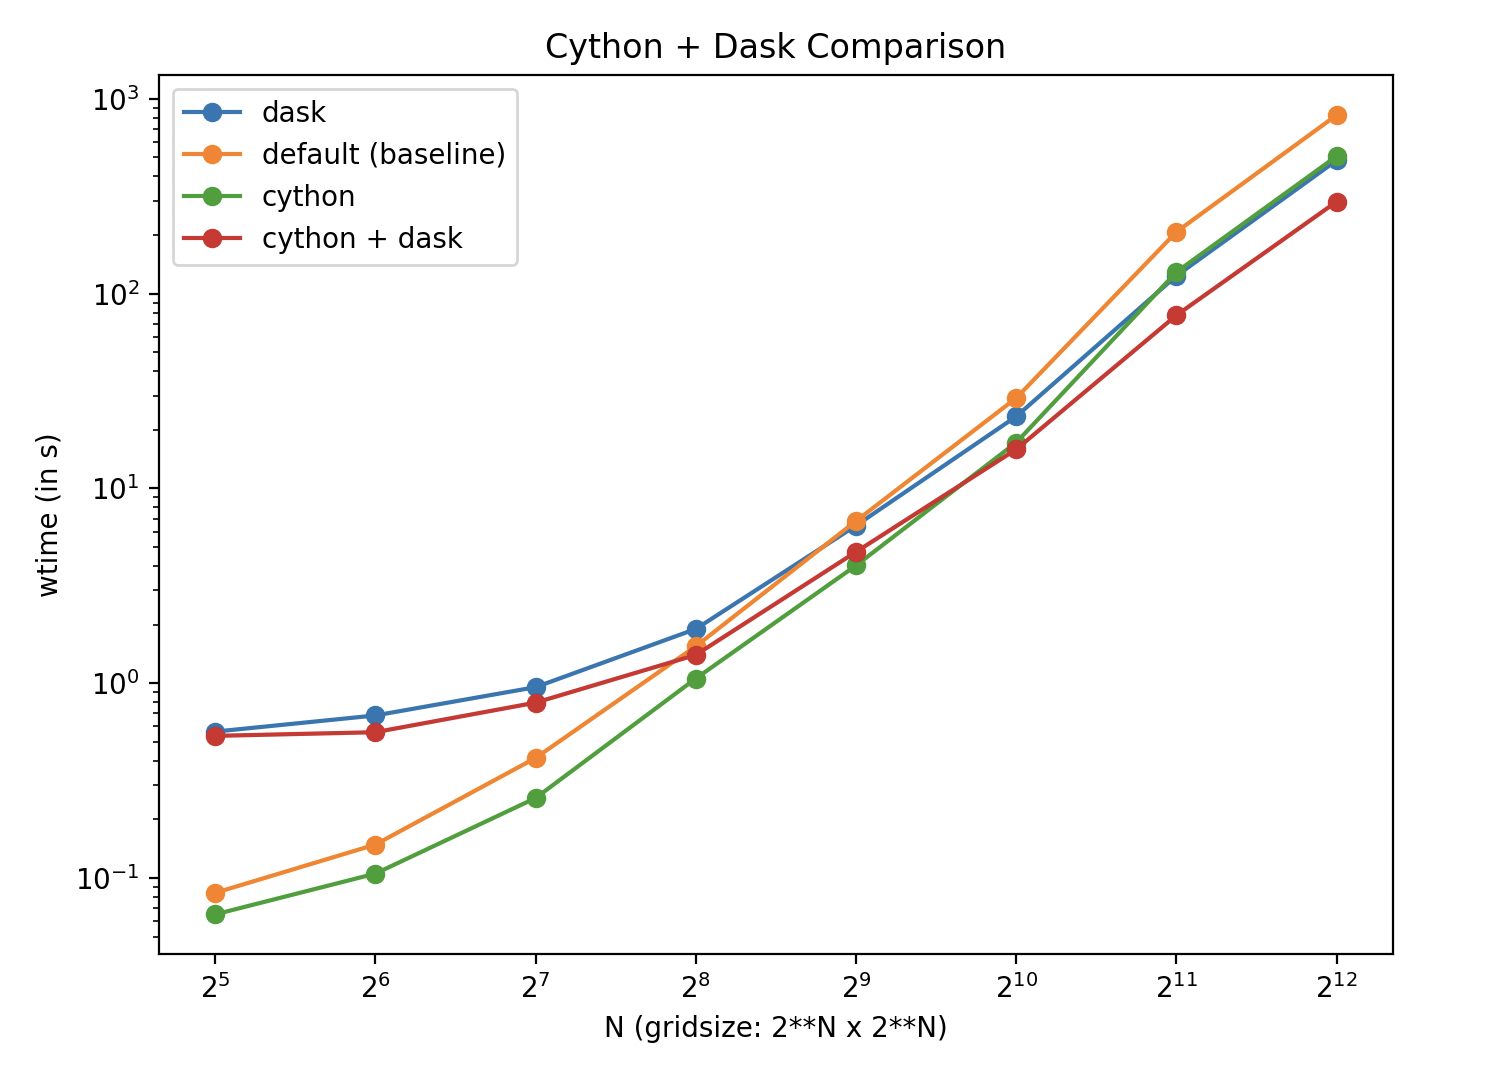
\includegraphics[width=\linewidth]{images/cython_dask/cython_dask_final_plot.png}
      \caption{Line Plot}
       \label{fig:cython_dask_final_plot}
   \end{minipage}
   \hspace{0.1cm}
   \begin{minipage}{0.5\textwidth}
       \centering
       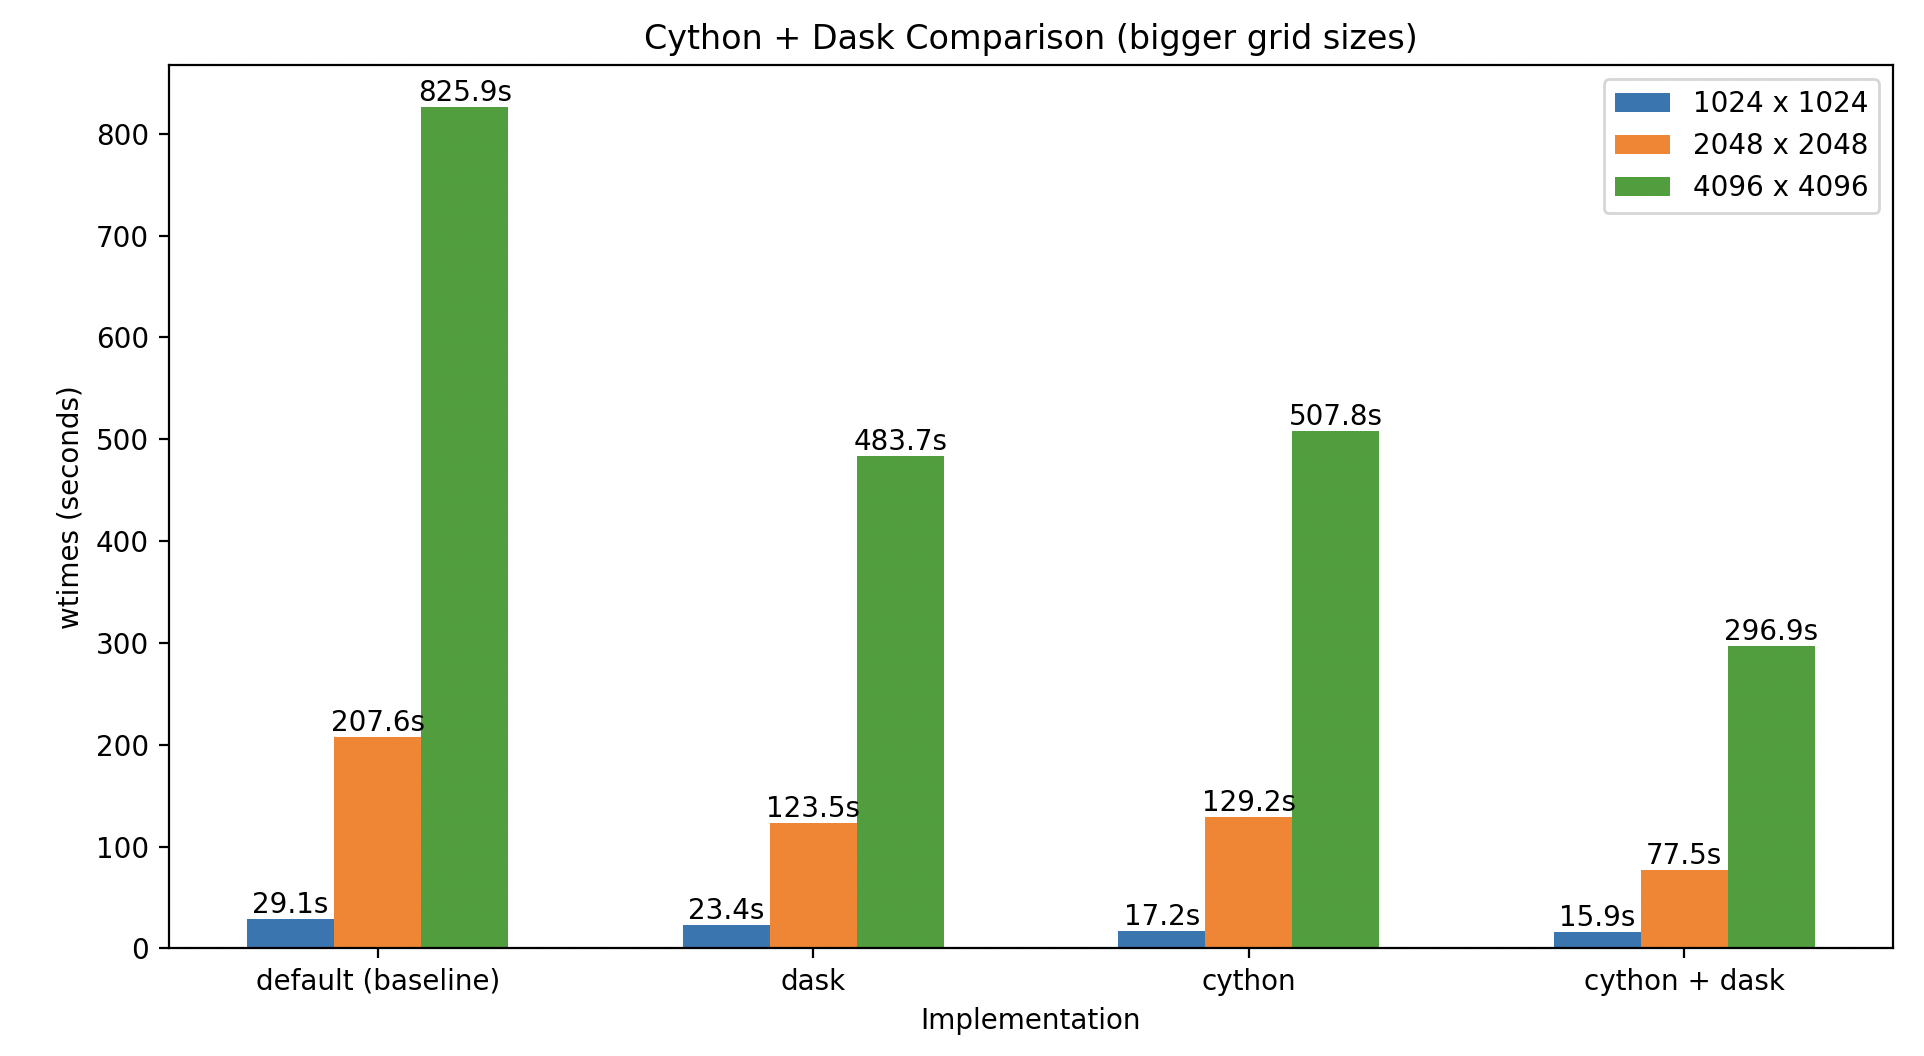
\includegraphics[width=\linewidth]{images/cython_dask/cython_dask_final_bar.png}
      \caption{Bar Graph}
      \label{fig:cython_dask_final_bar}
  \end{minipage}
  \caption{Cython + Dask Awesomeness}
\end{figure}

This lead to incredible results for larger grids, as can be seen in \ref{fig:cython_dask_final_plot}.
The combined approach outperforms the approaches of the individual optimizations, and of the baseline.
The bar graph in \ref{fig:cython_dask_final_bar} shows the runtimes in a non-lograithmic scale, highlighting the performance boost.
For smaller grids, this appears to be between the Cython and Dask optimizations.
This could be explained by the fact that the dask-overhead \textit{pulls up} the runtime compared to the sole Cython optimization, and the use of the optimized \verb|getFluxRawC| \textit{pulls down} the runtime compared compared to the sole Dask optimization.

\section{Conclusion}
The final plot of baseline runtime, and of all the \underline{chosen} optimizations, can be seen in Figure \ref{fig:final_plot}.
Figure \ref{fig:final_bar} shows the bar graphs for the largest 3 grid-sizes to highlight the performance improvements over the baseline.
\begin{figure}[h!]
   \begin{minipage}{0.5\textwidth}
       \centering
       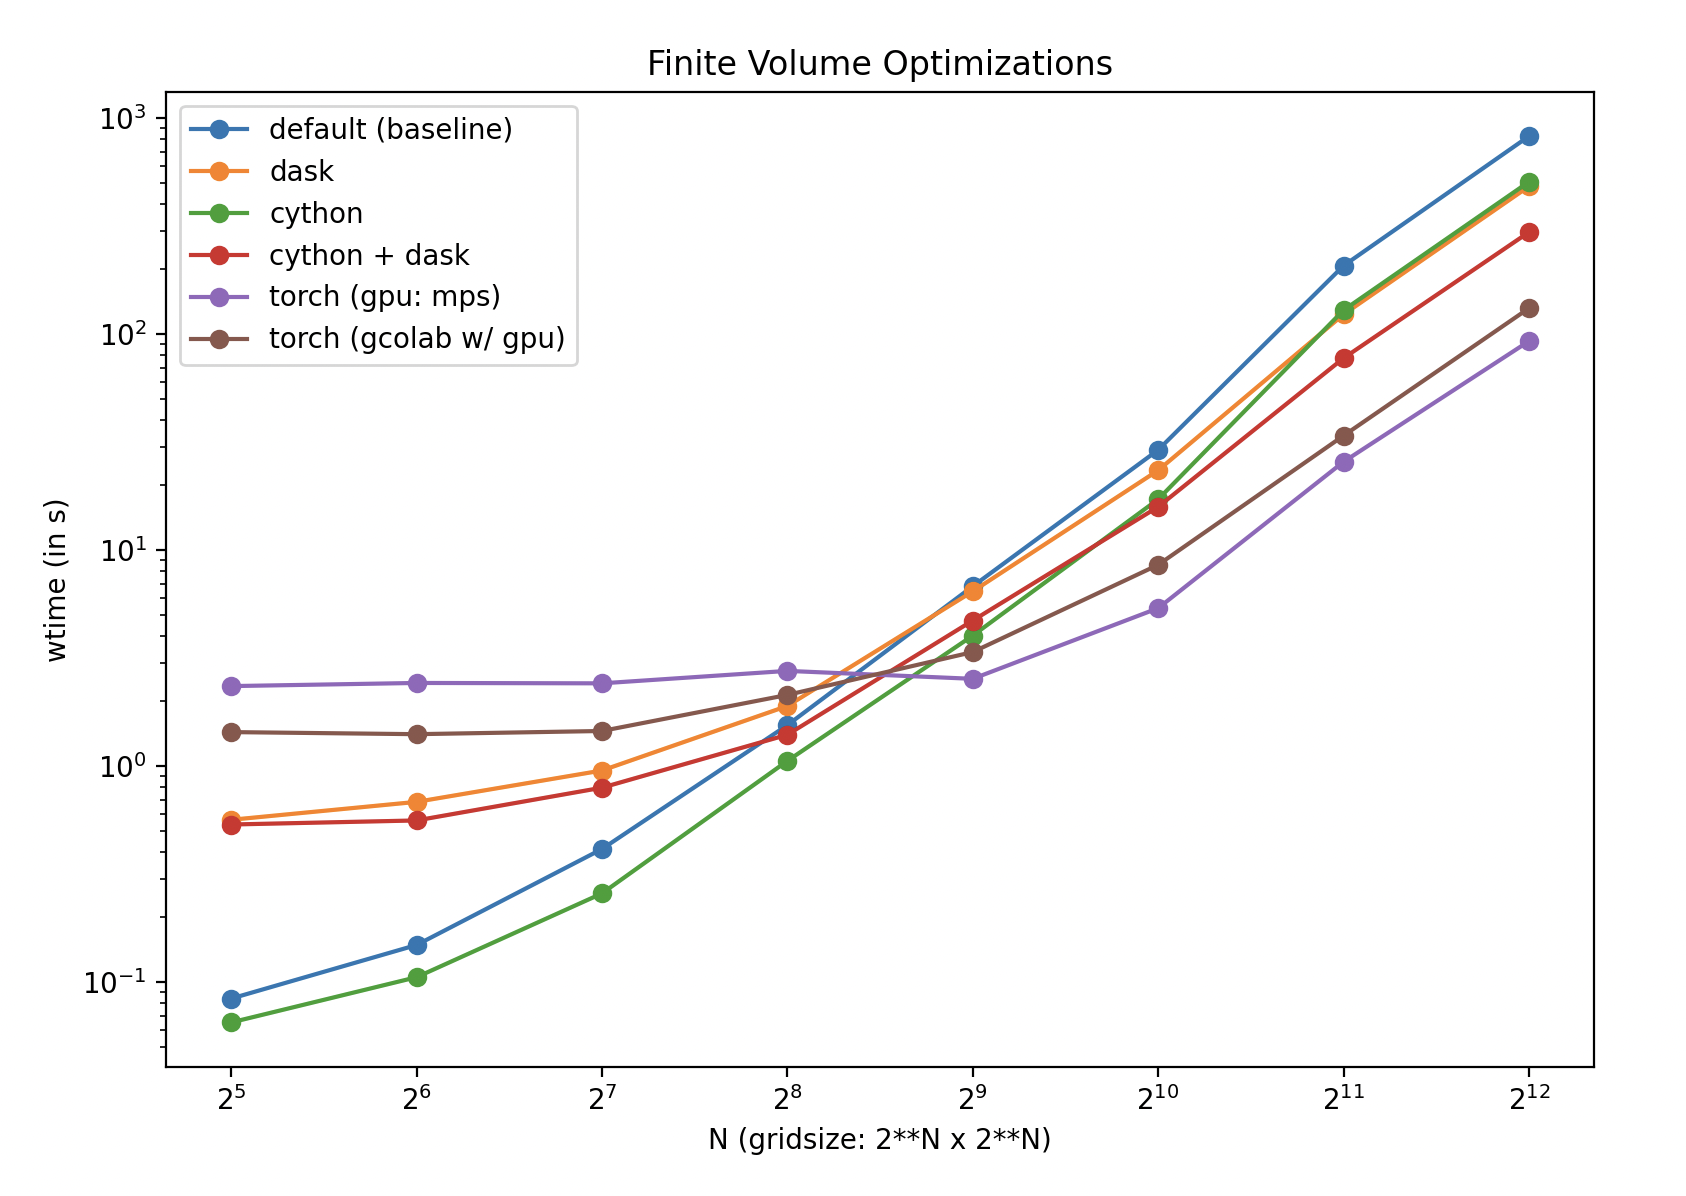
\includegraphics[width=\linewidth]{images/final/final_plot.png}
      \caption{Line Plot}
       \label{fig:final_plot}
   \end{minipage}
   \hspace{0.1cm}
   \begin{minipage}{0.5\textwidth}
       \centering
       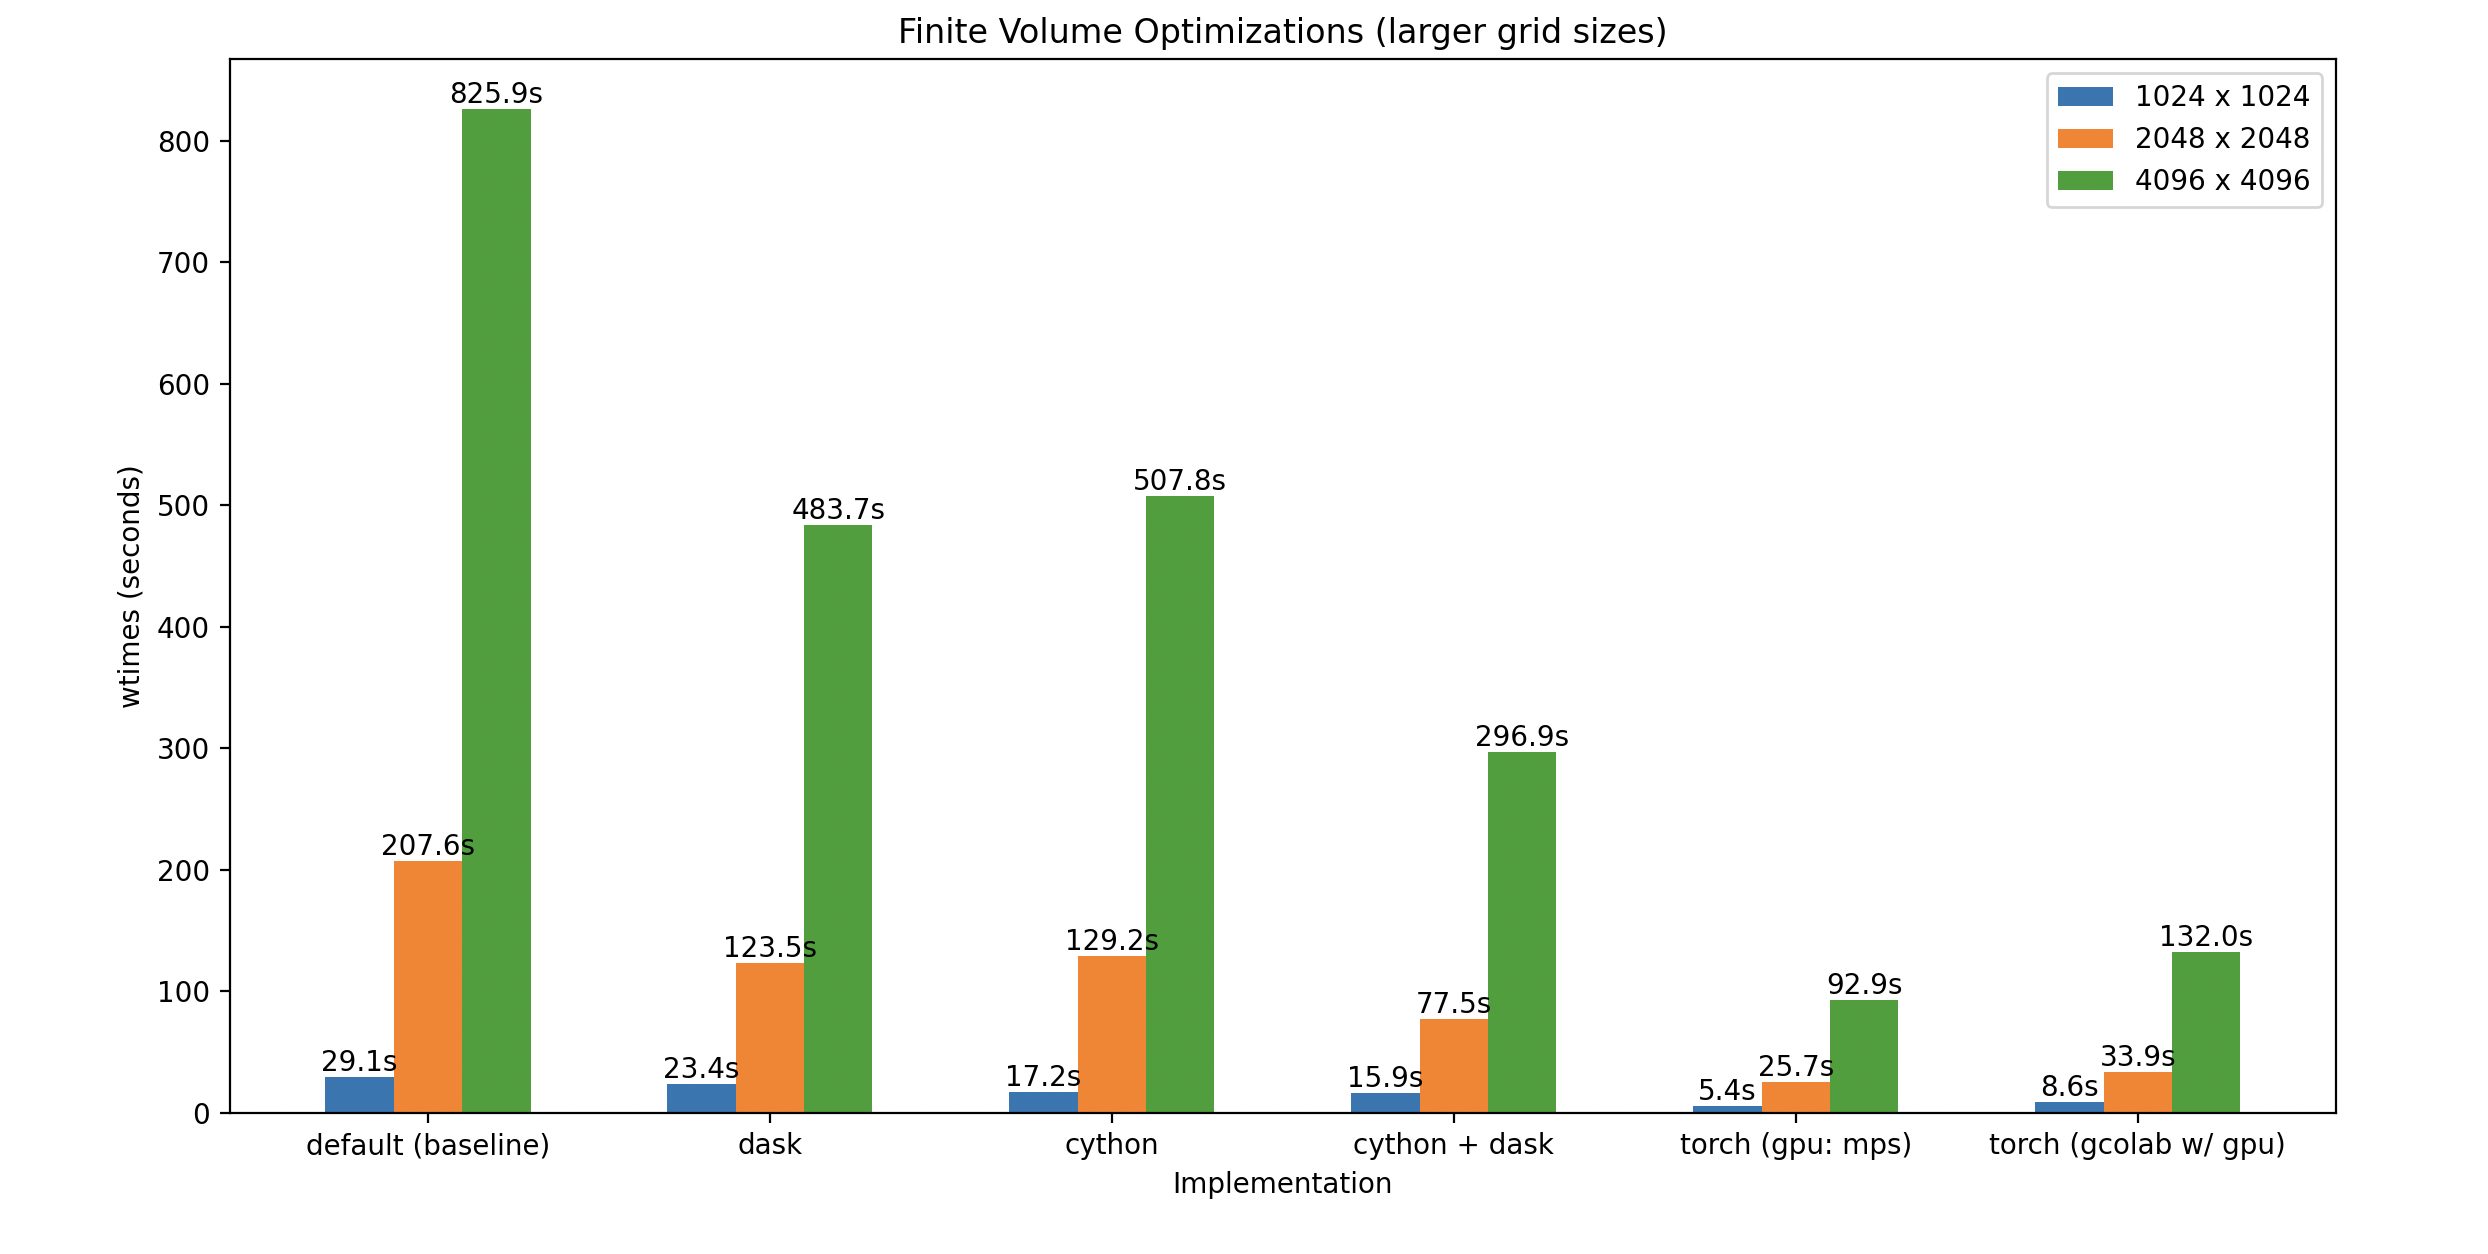
\includegraphics[width=\linewidth]{images/final/final_bar.png}
      \caption{Bar Graph}
      \label{fig:final_bar}
  \end{minipage}
  \caption{Cython + Dask Awesomeness}
\end{figure}
The trends and likely explanations for the trends observed in the runtime compared to the baseline have been discussed extensively in their respective sections.
Here, we would like to make one final important observation about the general trends.
For optimization approaches that require some overhead, whether it be initial or otherwise (such as moving data to the GPU, Dask-Delayed setup and \verb|compute()| calls, etc) -- approaches that work \textit{out of the box} without significant overhead seem to perform better (such as the Cython optimization and baseline).
However, the advantages of this \textit{hit} taken by such overhead starts becoming apparent when the grid-sizes increase.
This is when the sheer numbero of computations become overwhelming, and it helps the runtime to \textit{prepare} for such computations (with the overhead) and/or perform them in parallel: as can be seen by the better performance of the Dask, Dask with Cython, and the Torch implementations on larger grids.

\section{Appendix}

\subsection{Cython Attempt 3: Python Runtime Interactions}
\begin{figure}[H]
  \centering
  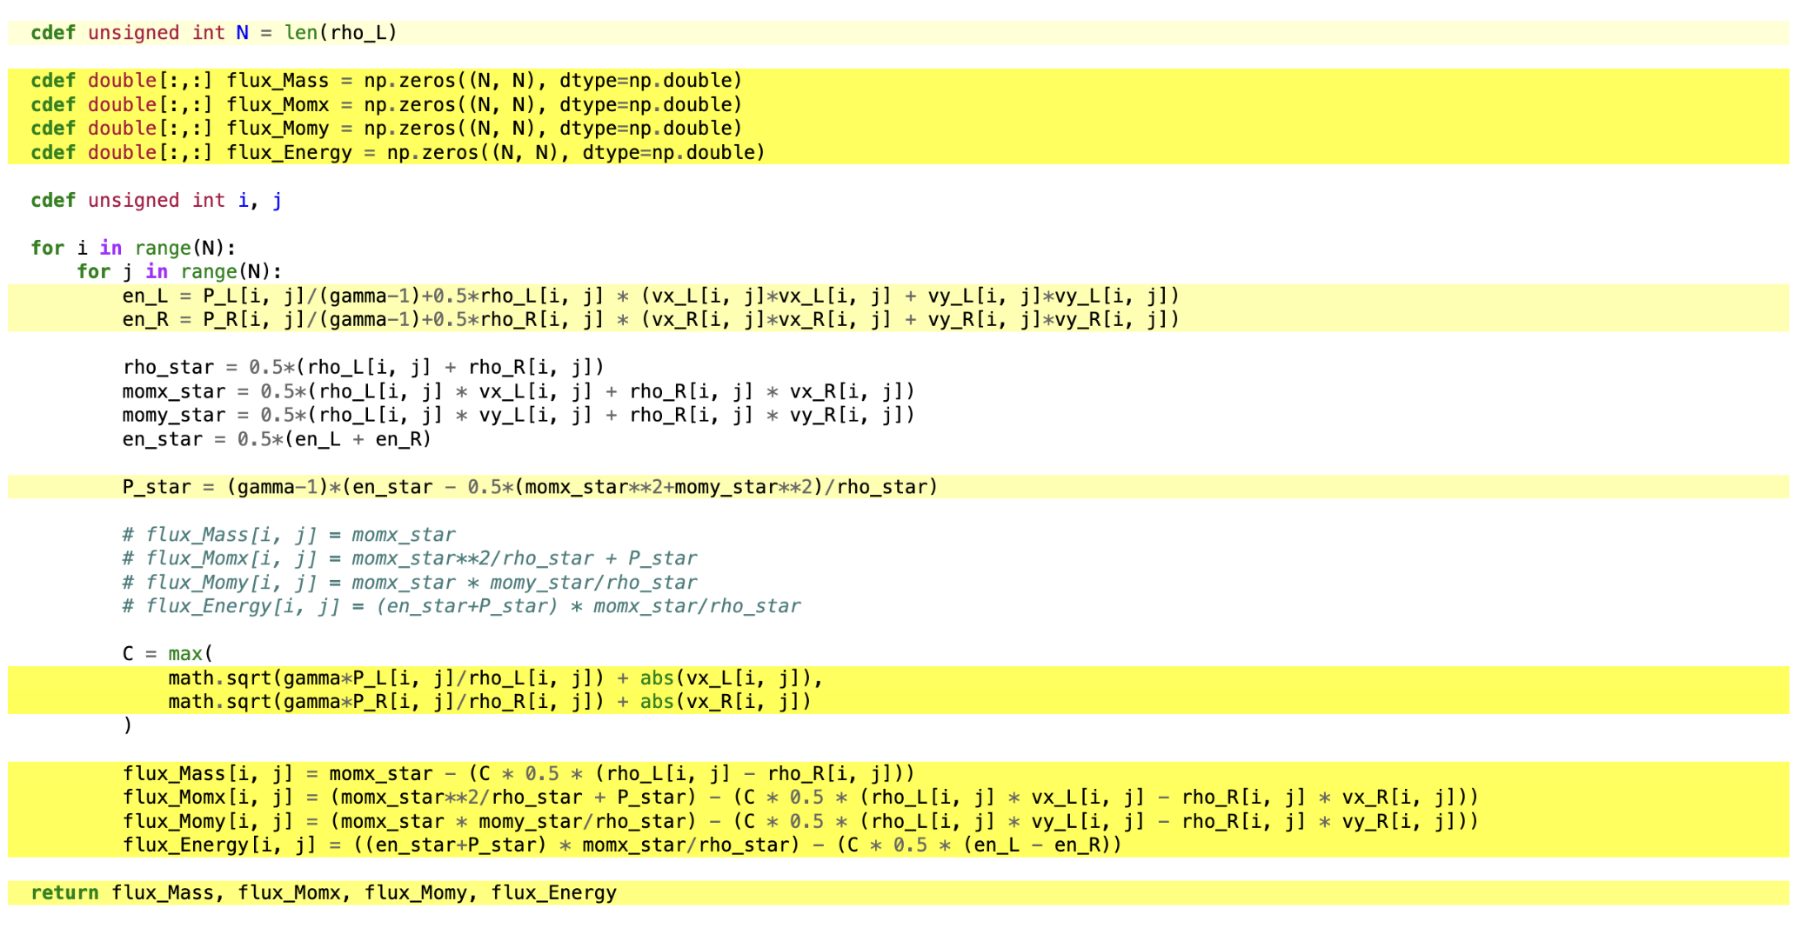
\includegraphics[width=0.9\textwidth]{images/misc/cython_attempt_3_annotated.png}
  \caption{Python Runtime Interactions for Cython Attempt 3}
  \label{fig:cython_attempt_3_annotated}
\end{figure}

\subsection{Dask Attempt 1: Dask Arrays Chunk Sizes Variation}
\begin{figure}[H]
  \centering
  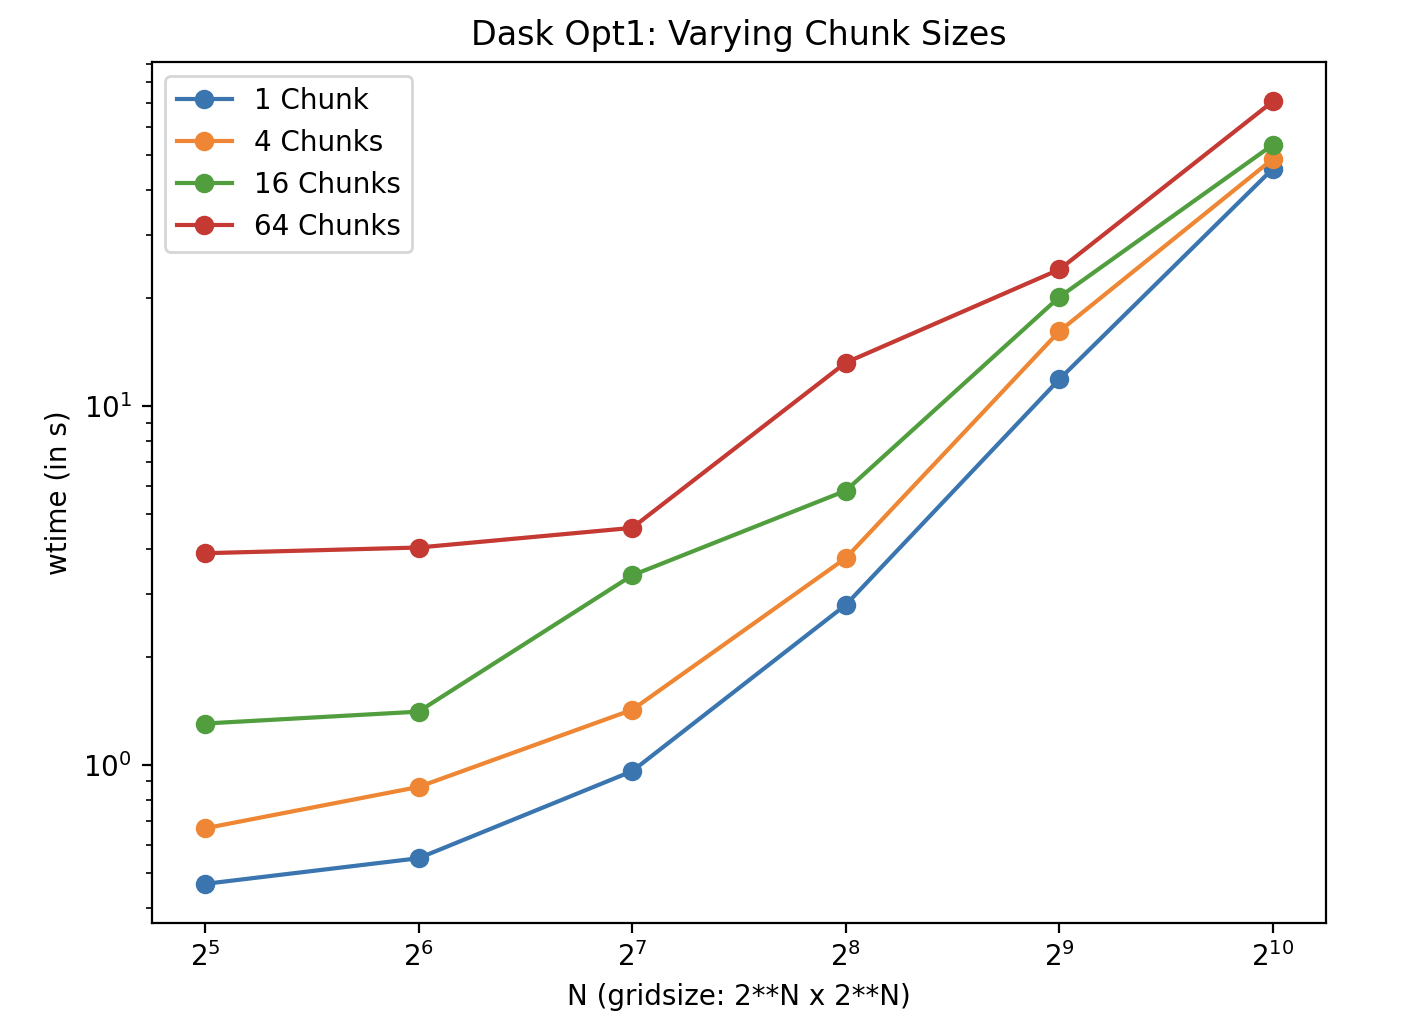
\includegraphics[width=0.9\textwidth]{images/dask/dask_opt1_chunk_size.png}
  \caption{Dask Attempt 1: Chunk Size Variation}
  \label{fig:dask_opt1_chunk_size}
\end{figure}

% content end
%###############################################################################

% TODO: bibliograpghy when needed
% \printbibliography

\end{document}
